\documentclass[12pt]{article}

\usepackage[utf8]{inputenc}
\usepackage{mwe}
\usepackage{graphicx}
\usepackage{epsfig}
\usepackage{cite}
\usepackage{geometry}
\usepackage{float}
\usepackage{subfig}
\usepackage{comment}
\usepackage[usenames,dvipsnames]{xcolor}

\usepackage[T1]{fontenc}
\usepackage{hyperref}
\usepackage{listings}
\usepackage{minted}



\definecolor{vgreen}{RGB}{104,180,104}
\definecolor{vblue}{RGB}{49,49,255}
\definecolor{vorange}{RGB}{255,143,102}


\lstdefinestyle{verilog-style}
{
    language=Verilog,
    frame=single,
    linewidth=17cm,
    basicstyle=\small\ttfamily,
    keywordstyle=\color{vblue},
    identifierstyle=\color{black},
    commentstyle=\color{vgreen},
    moredelim=*[s][\colorIndex]{[}{]},
    literate=*{:}{:}1
}

\lstdefinelanguage{VHDL}{
   morekeywords=[1]{
     LIBRARY,USE,ENTITY,IS,PORT,IN,OUT,END,ARCHITECTURE,OF,
     BEGIN,DOWNTO,ALL,WAIT,FOR,OTHERS,SIGNAL,PROCESS,WHEN,CASE,IF,ELSEIF,THEN
   },
   morekeywords=[2]{
     STD_LOGIC_VECTOR,STD_LOGIC,IEEE,STD_LOGIC_1164,
     NUMERIC_STD,STD_LOGIC_ARITH,STD_LOGIC_UNSIGNED,std_logic_vector,AND,OR,NOT,NAND,NOR,XOR,BIT_VECTOR,BIT,sll,srl,
     std_logic
   },
   morecomment=[l]--
}
\colorlet{keyword}{blue!100!black!80}
\colorlet{STD}{Lavender}
\colorlet{comment}{green!80!black!90}
\lstdefinestyle{vhdl}{
   language     = VHDL,
   basicstyle   = \footnotesize \ttfamily,
   keywordstyle = [1]\color{keyword}\bfseries,
   keywordstyle = [2]\color{STD}\bfseries,
   commentstyle = \color{comment}
}

\makeatletter
\newcommand*\@lbracket{[}
\newcommand*\@rbracket{]}
\newcommand*\@colon{:}
\newcommand*\colorIndex{%
    \edef\@temp{\the\lst@token}%
    \ifx\@temp\@lbracket \color{black}%
    \else\ifx\@temp\@rbracket \color{black}%
    \else\ifx\@temp\@colon \color{black}%
    \else \color{vorange}%
    \fi\fi\fi
}
\makeatother

\usepackage{trace}

\lstset{columns=fullflexible}

\begin{titlepage}
	\centering

    
    \textsc{\LARGE Implementation of Universal Shift Register in Verilog HDL/VHDL}\\[2.0 cm]

\begin{figure}[!htb]
\centering
  
\includegraphics[width=3cm,keepaspectratio]{logo.png}\textbf{ }\textbf{  }
  
\includegraphics[width=3cm,keepaspectratio]{download.png}\textbf{  }
  
\includegraphics[width=3cm,keepaspectratio]{modelsim-logo.jpg}
\end{figure}\\[2.0 cm]	
	\begin{minipage}{0.4\textwidth}
		\begin{flushleft} \large
			\emph{Mentors}\\
			Prasad T\\
            Aditya Gudla\\
            Simranjeet Singh \
			\end{flushleft}
			\end{minipage}~
			\begin{minipage}{0.4\textwidth}
            
			\begin{flushright} \large
			\emph{Interns} \\
			Ajay Chaudhari\\
            Chethan T Bhat\\
            Ritvik Tiwari \\
            Karthik A Shet \\
		\end{flushright}
	\end{minipage}\\[2 cm]
\end{titlepage}

\begin{document}
\tableofcontents
\newpage

\section{Introduction}
\subsection{What is a Register?}

Flip flops can be used to store a single bit of binary data (1 or 0). However, in order to store multiple bits of data, we need multiple flip flops. N flip flops are to be connected in an order to store n bits of data. A \textbf{Register} is a device which is used to store such information. It is a group of flip flops connected in series used to store multiple bits of data.

\subsection{Shift Registers}
The information stored within these registers can be transferred with the help of \textbf{Shift Registers}. Shift Register is a group of flip flops used to store multiple bits of data. The bits stored in such registers can be made to move within the registers and in/out of the registers by applying clock pulses. An n-bit shift register can be formed by connecting n flip-flops where each flip flop stores a single bit of data.
\\
\noindent Shift registers are basically of 4 types. These are: 
\begin{enumerate}
    \item Serial In Serial Out shift register
    \item Serial In parallel Out shift register
    \item Parallel In Serial Out shift register
    \item Parallel In parallel Out shift register

\end{enumerate}

\subsection{Serial-In Serial-Out Shift Register}
The shift register, which allows serial input (one bit after the other through a single data line) and produces a serial output is known as Serial-In Serial-Out shift register. Since there is only one output, the data leaves the shift register one bit at a time in a serial pattern, thus the name Serial-In Serial-Out Shift Register.

\noindent The logic circuit given below shows a serial-in serial-out shift register. The circuit consists of four D flip-flops which are connected in a serial manner. All these flip-flops are synchronous with each other since the same clock signal is applied to each flip flop.
\begin{figure}[H]
    \centering
    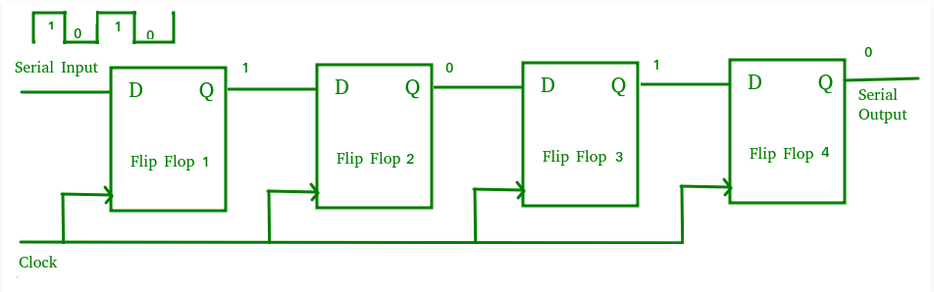
\includegraphics[scale=0.6]{circuit diagram/SISO.png}
    \caption{SISO Shift Register}
\end{figure}
\subsection{Serial-In Parallel-Out Shift Register}
The shift register, which allows serial input (one bit after the other through a single data line) and produces a parallel output is known as Serial-In Parallel-Out shift register.

\noindent The logic circuit given below shows a serial-in-parallel-out shift register. The circuit consists of four D flip-flops which are connected. The clear (CLR) signal is connected in addition to the clock signal to all the 4 flip flops in order to RESET them. The output of the first flip flop is connected to the input of the next flip flop and so on. All these flip-flops are synchronous with each other since the same clock signal is applied to each flip flop.
\begin{figure}[H]
    \centering
    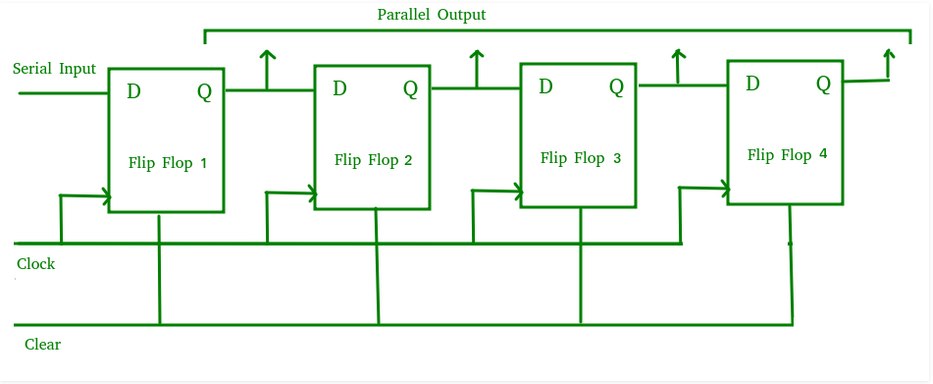
\includegraphics[scale=0.6]{circuit diagram/SIPO.png}
    \caption{SIPO Shift Register}
\end{figure}

\subsection{Parellel-In Serial-Out Shift Register}
The PISO(Parellel-in Serial-out) shift register has one of the most important application among the shift register, and it is to convert parellel data into serial data, which is extensively used in communication.

\noindent The circuit consists of four D flip-flops which are connected. The clock input is directly connected to all the flip flops but the input data is connected individually to each flip flop through a multiplexer at the input of every flip flop. The output of the previous flip flop and parallel data input are connected to the input of the MUX and the output of MUX is connected to the next flip flop. All these flip-flops are synchronous with each other since the same clock signal is applied to each flip flop.
\begin{figure}[H]
    \centering
    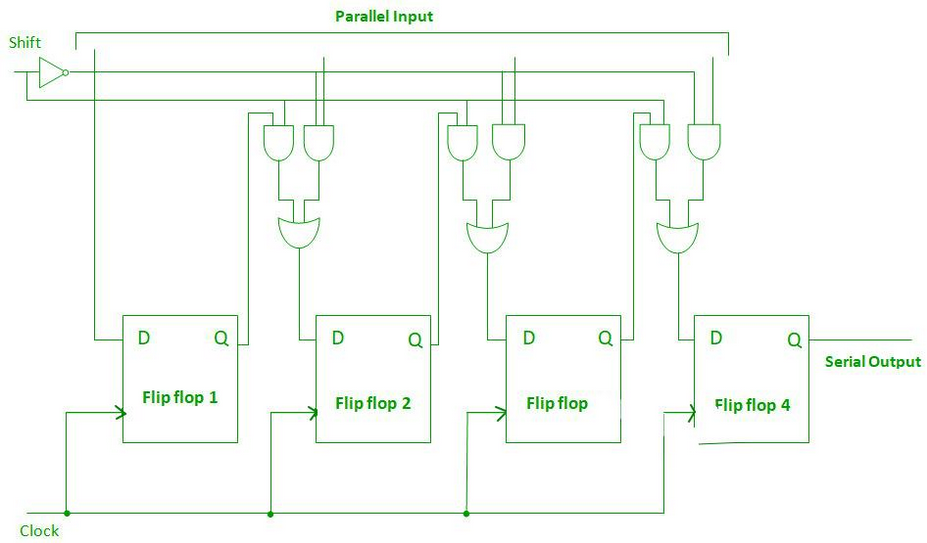
\includegraphics[scale=0.6]{circuit diagram/PISO.png}
    \caption{PISO Shift Register}
\end{figure}

\subsection{Parallel-In Parallel-Out Shift Register}
The shift register, which allows parallel input (data is given separately to each flip flop and in a simultaneous manner) and also produces a parallel output is known as Parallel-In parallel-Out shift register.

\noindent The logic circuit given below shows a parallel-in-parallel-out shift register. The circuit consists of four D flip-flops which are connected. The clear (CLR) signal and clock signals are connected to all the 4 flip flops. In this type of register, there are no interconnections between the individual flip-flops since no serial shifting of the data is required. Data is given as input separately for each flip flop and in the same way, output also collected individually from each flip flop.
\begin{figure}[H]
    \centering
    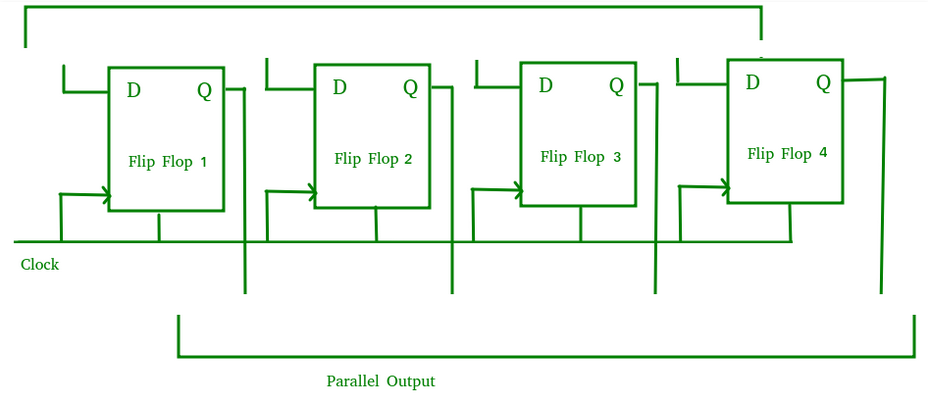
\includegraphics[scale=0.5]{circuit diagram/PIPO.png}
    \caption{PIPO Shift Register}
\end{figure}

\subsection{Universal Shift Register}
A Universal shift register is a register is a combination of all the above 4 shift registers with. Universal shift registers are used as memory elements in computers. A Unidirectional shift register is capable of shifting in only one direction. A bidirectional shift register is capable of shifting in both the directions. The Universal shift register is a combination design of bidirectional shift register and a unidirectional shift register with parallel load provision.
\begin{figure}[H]
    \centering
    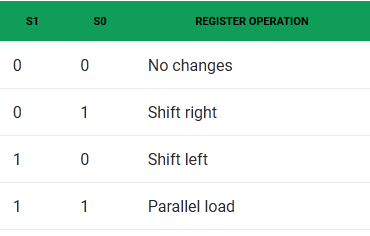
\includegraphics[]{circuit diagram/uni_operation.png}
    \caption{Choosing the operation through MUX select lines}
\end{figure}
\begin{figure}[H]
    \centering
    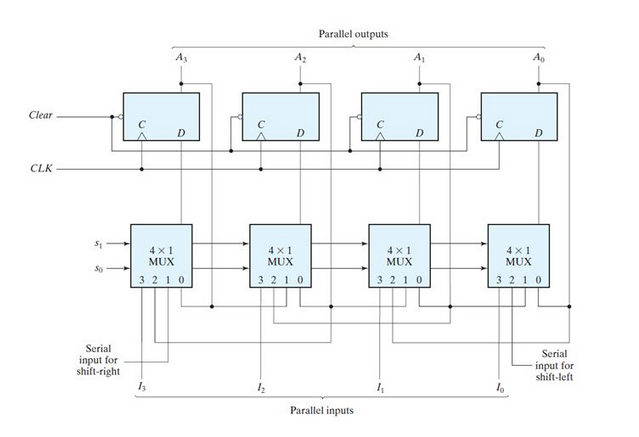
\includegraphics[scale=0.8]{circuit diagram/universal.png}
    \caption{Universal Shift Register}
    \label{fig:univ}
\end{figure}

\newpage
\section{Verilog HDL Code for Universal Shift Register}
The Universal Shift Register has been implemented as it contains all different types of shift registers in itself.
\subsection{RTL Description}
\begin{lstlisting}[style=verilog-style]
module Universal_Shift_Register_Verilog(
	input [3:0]i,   //Define pins for parellel input
	input [1:0]sel,	//Define select line pins to choose the operation
	input clk,rst,il,ir,  //Define clock,reset, serial input for 
	                    //shift left and serial input for shift right
	output reg [3:0]out_bit); //Define output pins
	


always @ (posedge clk, negedge rst ) //Execute the logic whenever positive edge of  
                                     //clock or negative edge of Reset is encountered
begin
	if(rst==0)    //if rst = 0, then clear the output
		out_bit=4'b000;
	else
	begin
		case(sel)  //check select lines to determine type of 
		         //operation
			2'b00:begin end //Retain the data
			2'b01:begin
				out_bit={ir,out_bit[3:1]}; //shift right operation
				end
			2'b10:begin
				out_bit={out_bit[2:0],il}; //Shift left operation
				end
			2'b11:begin
				out_bit = i;  //parellel input-output operation
				end
			default:begin end
		endcase
	end
end
endmodule

\end{lstlisting}
\subsection{Testbench}
\begin{lstlisting}[style=verilog-style]
module Universal_Shift_Register_tb;
reg [3:0]i; reg[1:0]sel; reg clk; reg rst; reg il;reg ir; //Define all input ports
wire [3:0]out_bit;  //Define all output ports

Universal_Shift_Register_Verilog uut(.i(i),    //Map testbench ports with DUT ports
                       .sel(sel),
					   .clk(clk),
					   .rst(rst),
					   .out_bit(out_bit),
					   .il(il),
					   .ir(ir));

initial begin   

	rst = 1'b0;  //Initialze values on all input pins
	clk = 0;
	ir = 0;
	il = 0;
	sel = 2'b00;
	i = 4'b0000;
end

always
begin			
	clk = ~clk; #5;	//Define Clock operation
end

initial begin
	#50;
	rst = 1; #50	//Different Combinations of input
	ir = 1;
	sel = 2'b01;#10;
	ir = 0;#10;
	ir = 1;#10;
	ir = 0;#10;
	il = 1;
	sel = 2'b00;#50
	sel = 2'b10;
	il = 1;#10
	il = 0;#10
	il = 0;#10
	sel = 2'b11;#5
	i = 4'b1111;
	#100;
end
endmodule
	

\end{lstlisting}

\newpage
\section{Implementation in Quartus Prime}
To Implement the design in Quartus Software, follow these steps(For more detailed information on the following steps, Refer '\textbf{Quick Start Guide to Quartus Prime Lite & ModelSim}' Document):

\noindent \textbf{Note:} The language used is Verilog HDL. Device is DE0-Nano FPGA Board
\begin{enumerate}
    \item Create a New Project using the Project Wizard.
    \begin{figure}[H]
        \centering
        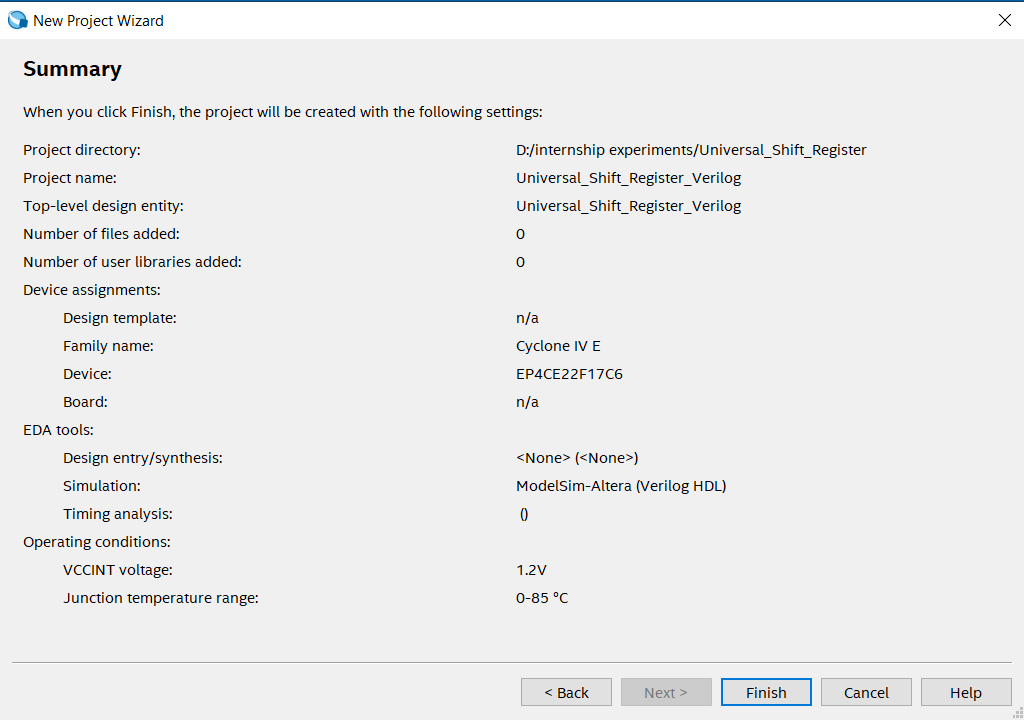
\includegraphics[scale=0.7]{USR1.png}
        \caption{Project Summary}
    \end{figure}
    \item Create a New Verilog File
    \begin{figure}[H]
        \centering
        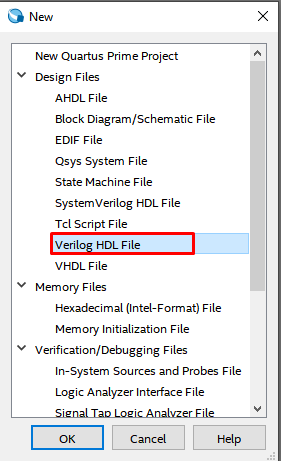
\includegraphics[scale=0.5]{Implementation_quartus/2.png}
        \caption{Creating a Verilog File}
    \end{figure}
    \item Type in the Verilog code provided in this Document and save the file(make sure file name is same as module name)
    \begin{figure}[H]
        \centering
        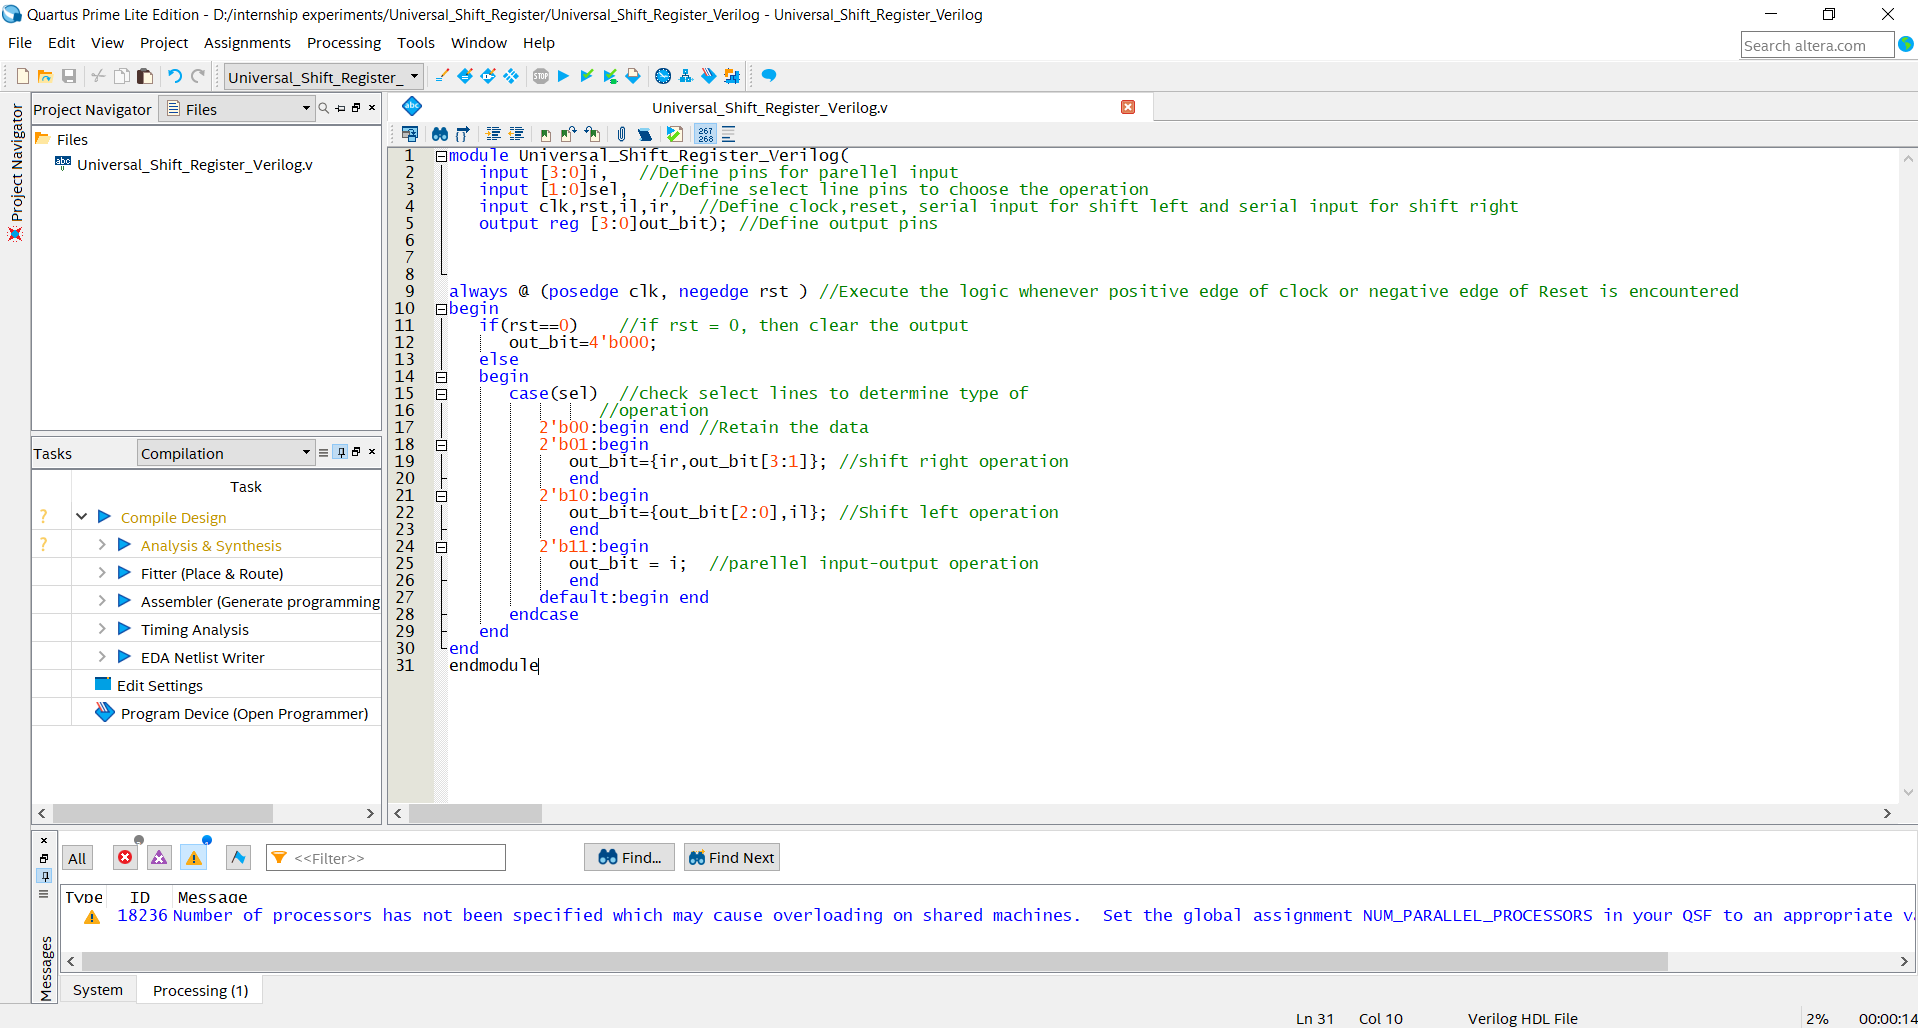
\includegraphics[scale=0.4]{USR2.png}
        \caption{Code typed and saved}
    \end{figure}
    
    \textbf{Note:}If module name is different from project name, then manually set the verilog file as Top-Level Module by:Right Click on \textbf{'<File\_name>'$\rightarrow$Set as Top-Level Entity}
    \begin{figure}[H]
        \centering
        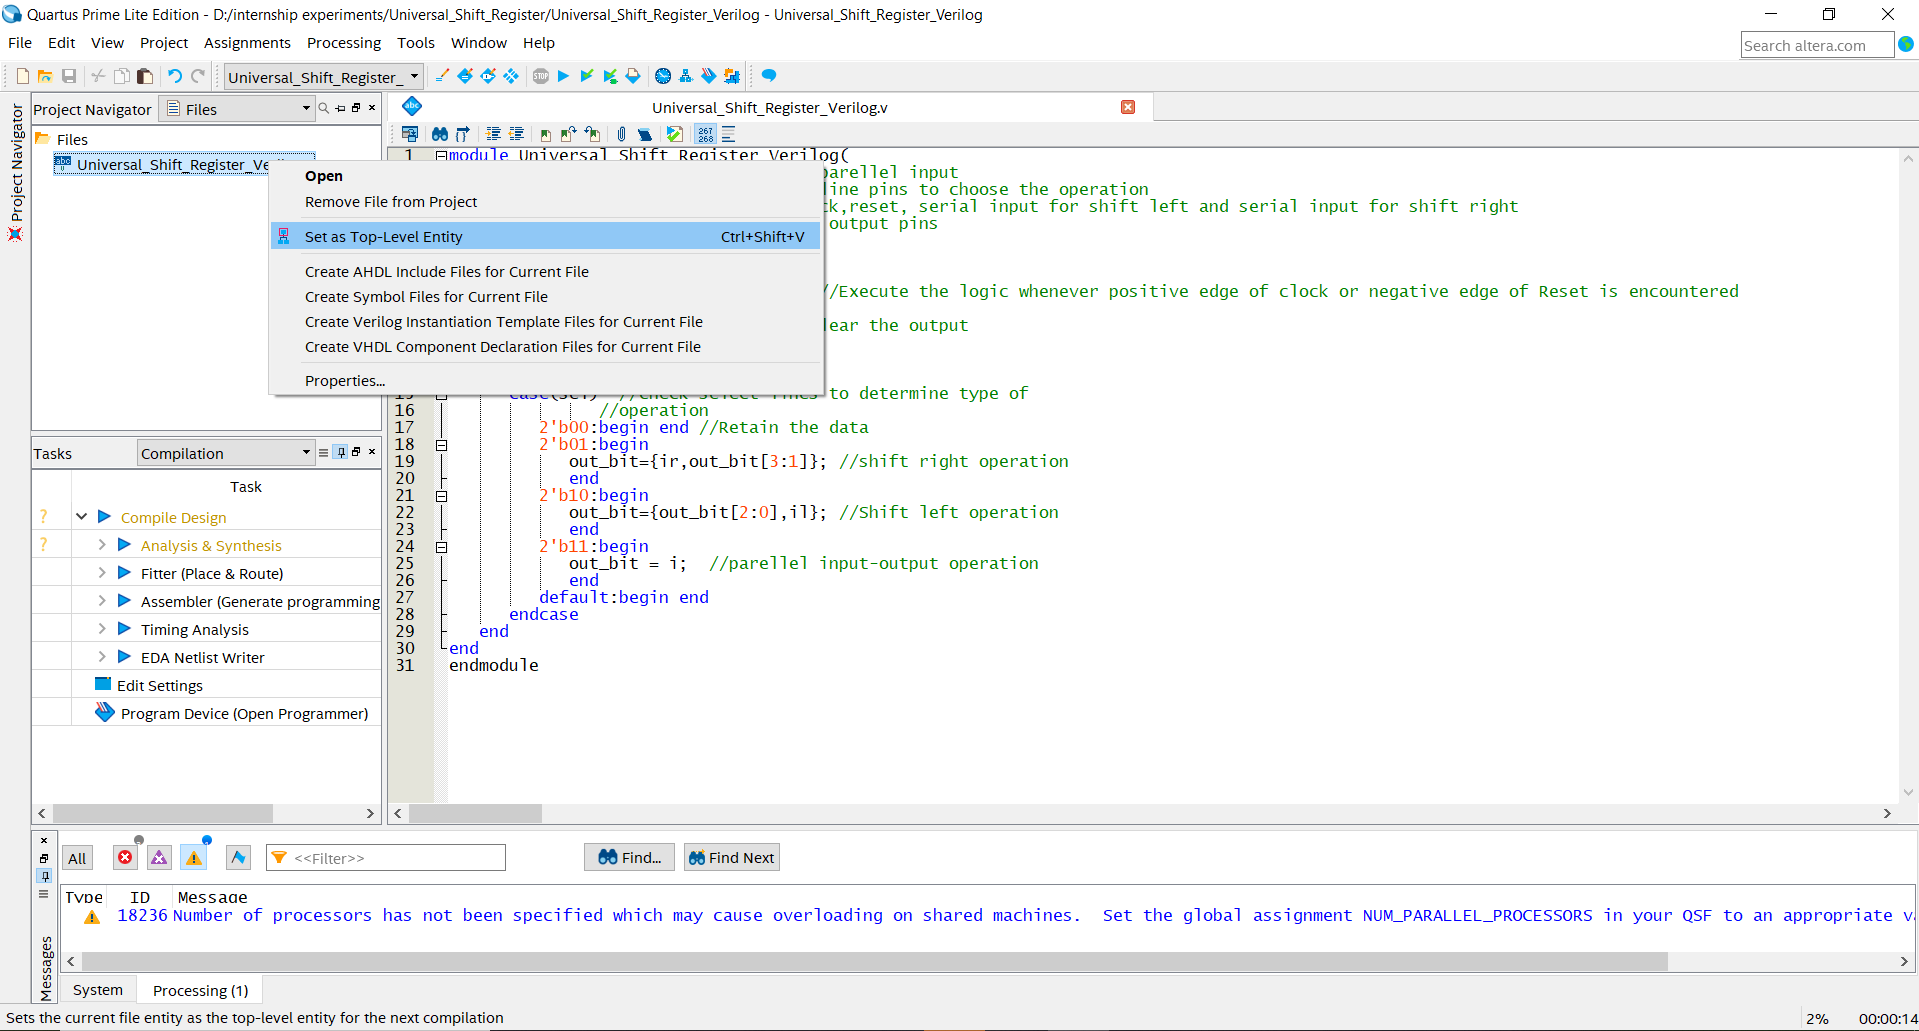
\includegraphics[scale=0.4]{USR3.png}
        \caption{Setting top-level entity}
    \end{figure}
    
    \item Compile the Design either by double clicking '\textbf{COMPILE DESIGN}' or clicking on the '\textbf{Play}' button
    \begin{figure}[H]
        \centering
        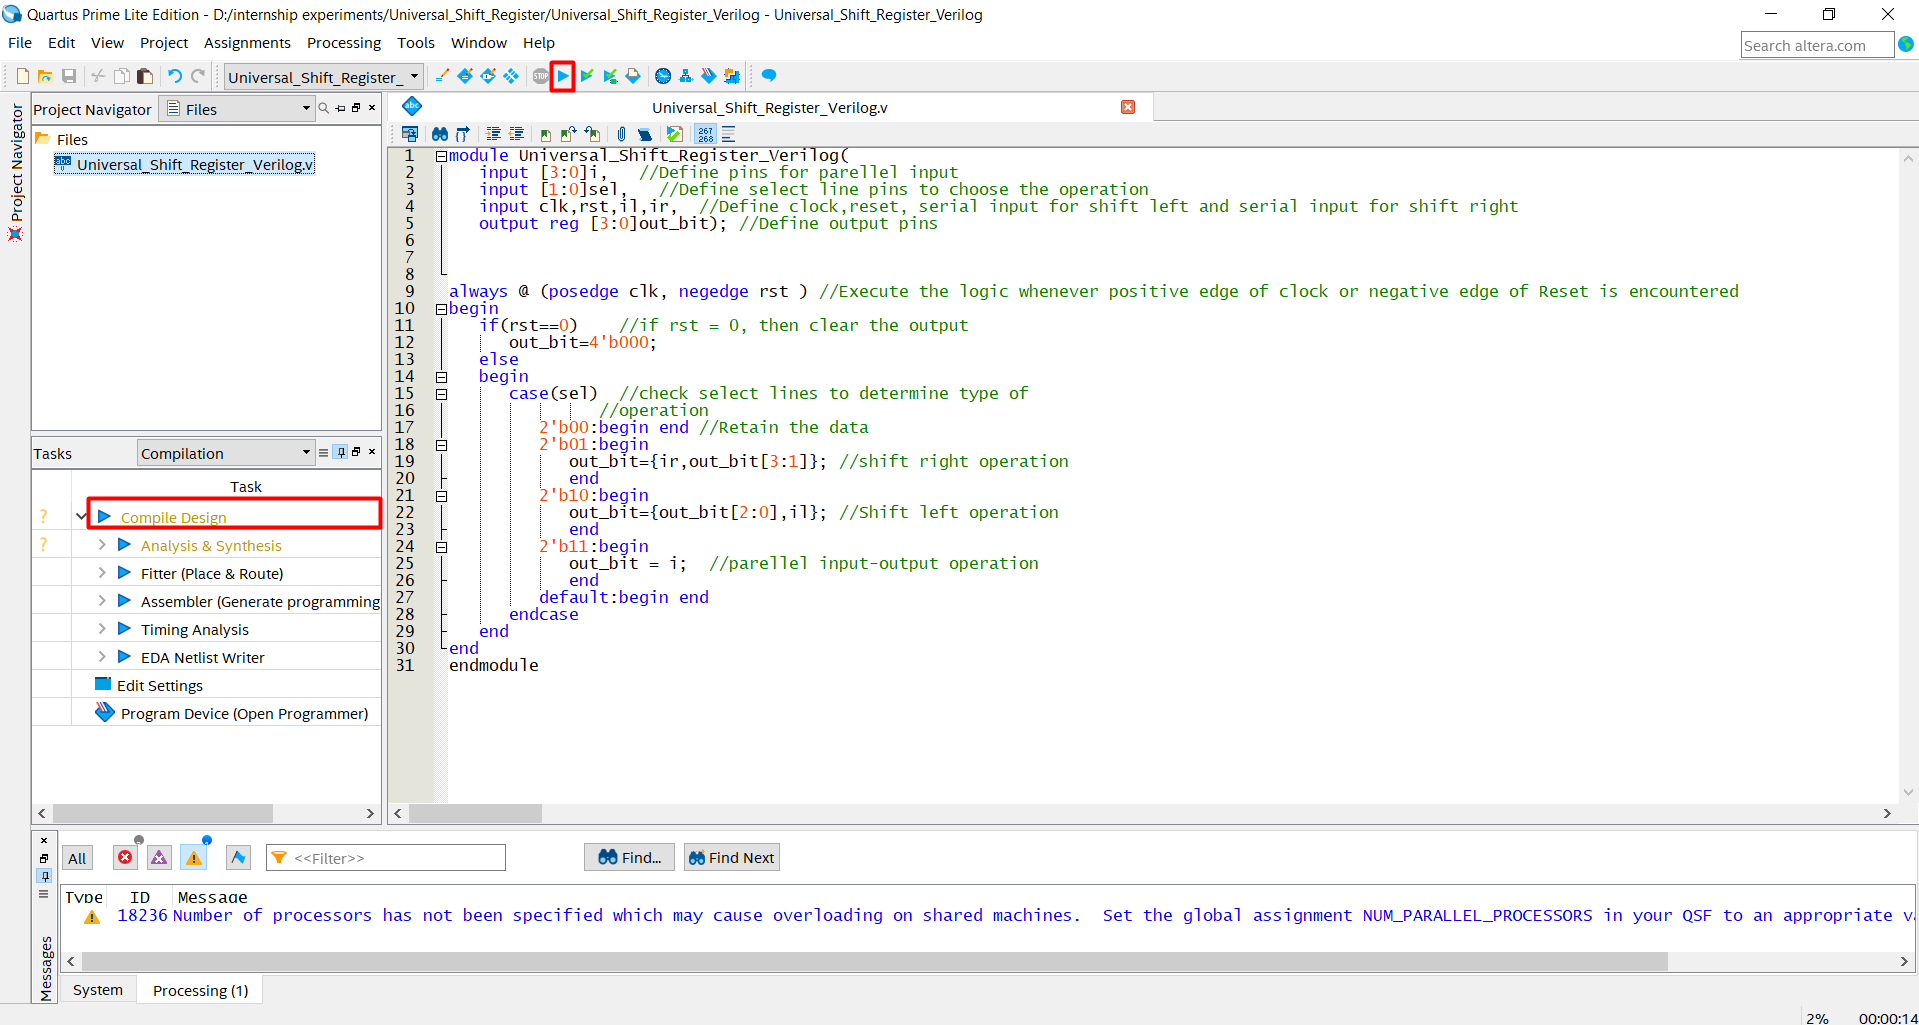
\includegraphics[scale=0.4]{USR4.png}
        \caption{Code compilation}
    \end{figure}
    \textbf{Note:}The Compilation is complete when you see these \textbf{Green Tick} marks.If even one of them have \textbf{Red Cross} it means the compilation has failed
    \begin{figure}[H]
        \centering
        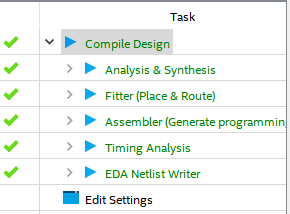
\includegraphics[scale=0.6]{Implementation_quartus/4_1.png}
        \caption{Successful compilation}
    \end{figure}
    
    \item Upon successful compilation,to view the RTL Circuit, Go to \textbf{TOOLS$\rightarrow$NETLIST VIEWERS$\rightarrow$RTL VIEWER}
    \begin{figure}[H]
        \centering
        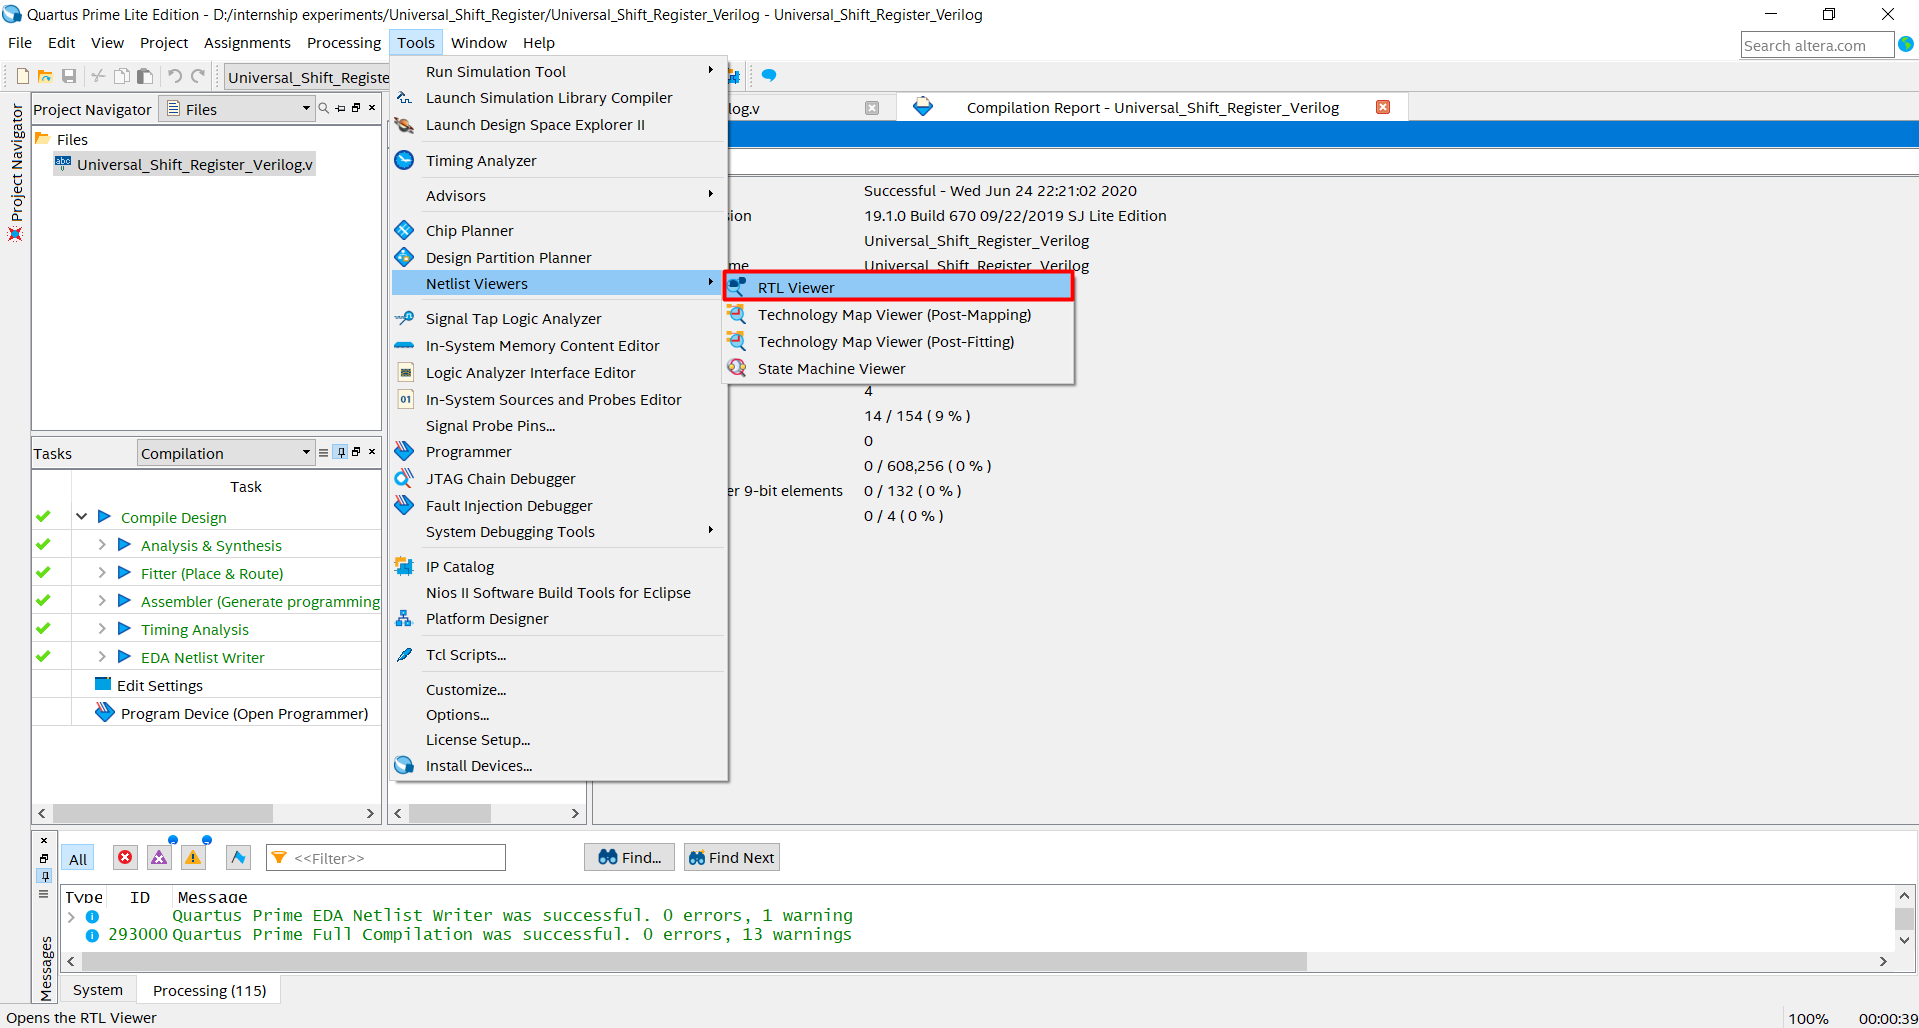
\includegraphics[width=14cm,keepaspectratio]{usr5.png}
        \caption{Opening the RTL Viewer}
    \end{figure}
\end{enumerate}



\section{RTL Circuit of the Implemented Design}
The below RTL circuit is the result of our design
\begin{figure}[H]
    \centering
    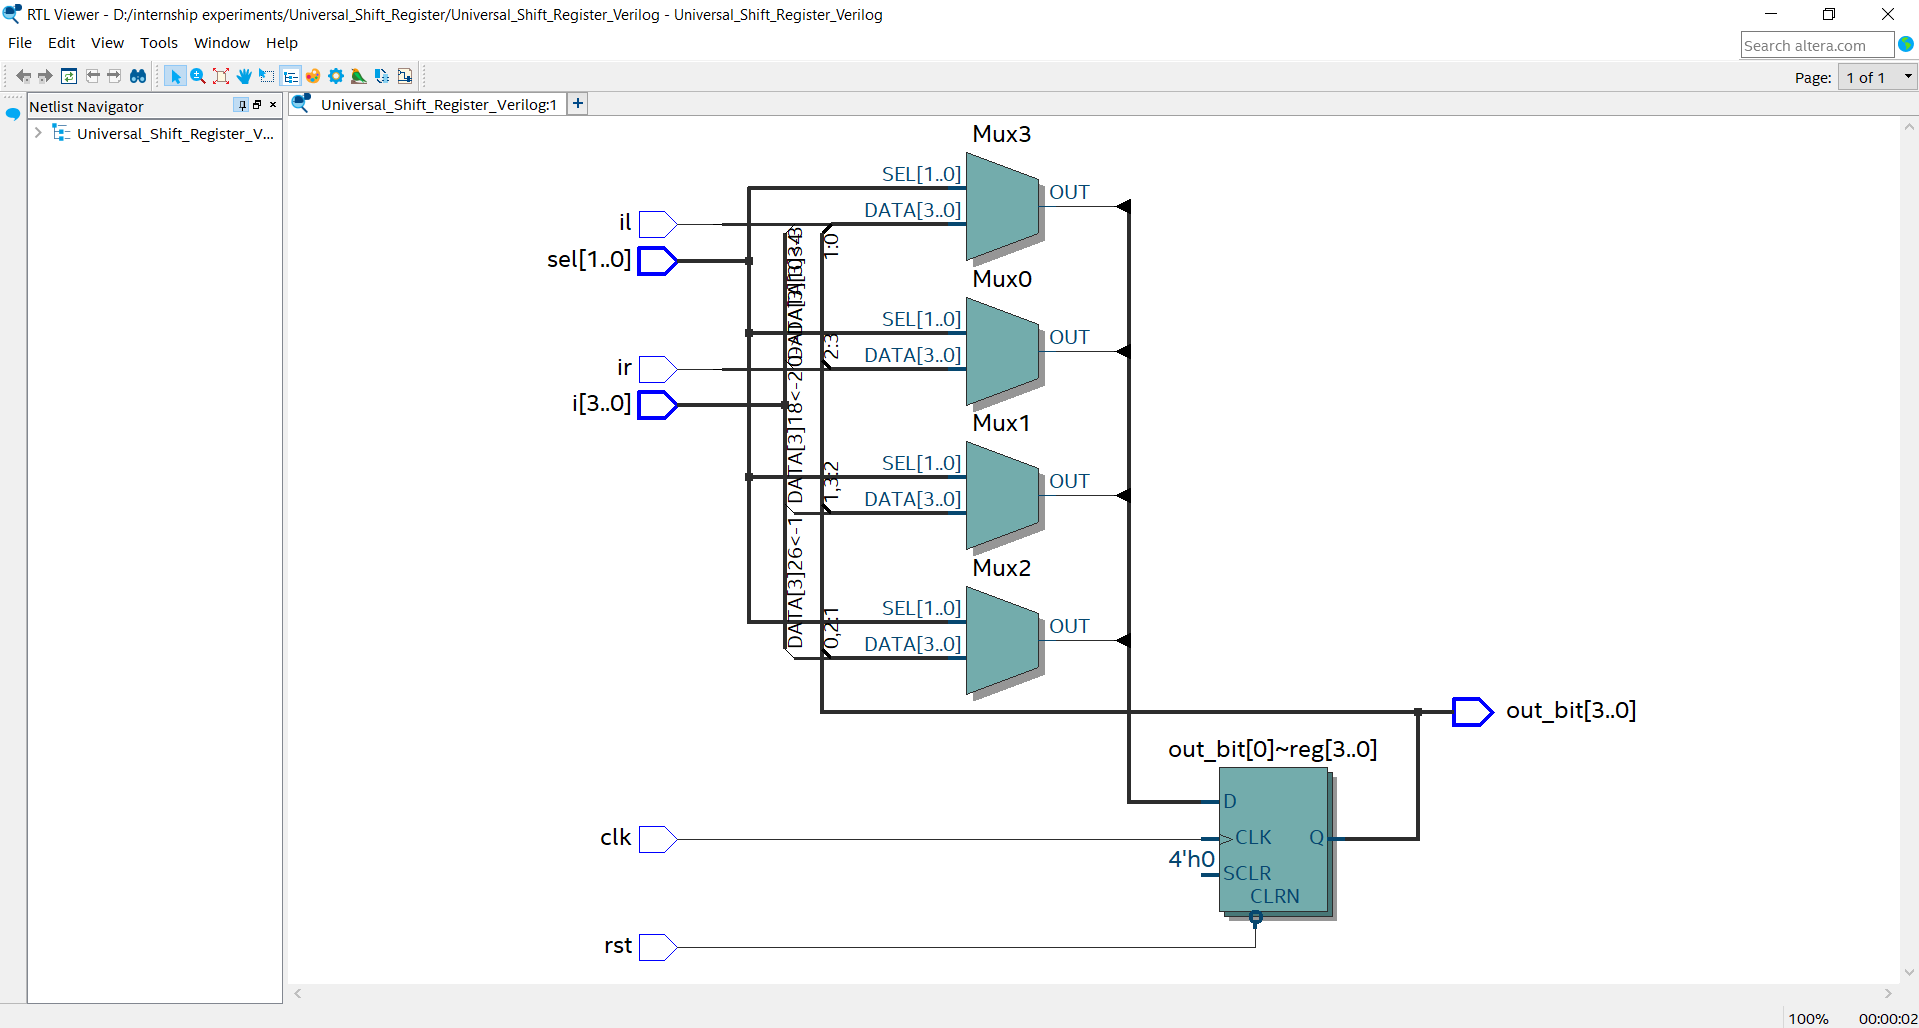
\includegraphics[width=14cm,keepaspectratio]{usr6.png}
    \caption{RTL Circuit of Universal Shift Register}
\end{figure}

\newpage
\section{Pin Assignment}
\begin{enumerate}
    \item Open the \textbf{Pin Planner} by going to \textbf{ASSIGNMENTS$\rightarrow$PIN PLANNER}
    \begin{figure}[H]
        \centering
        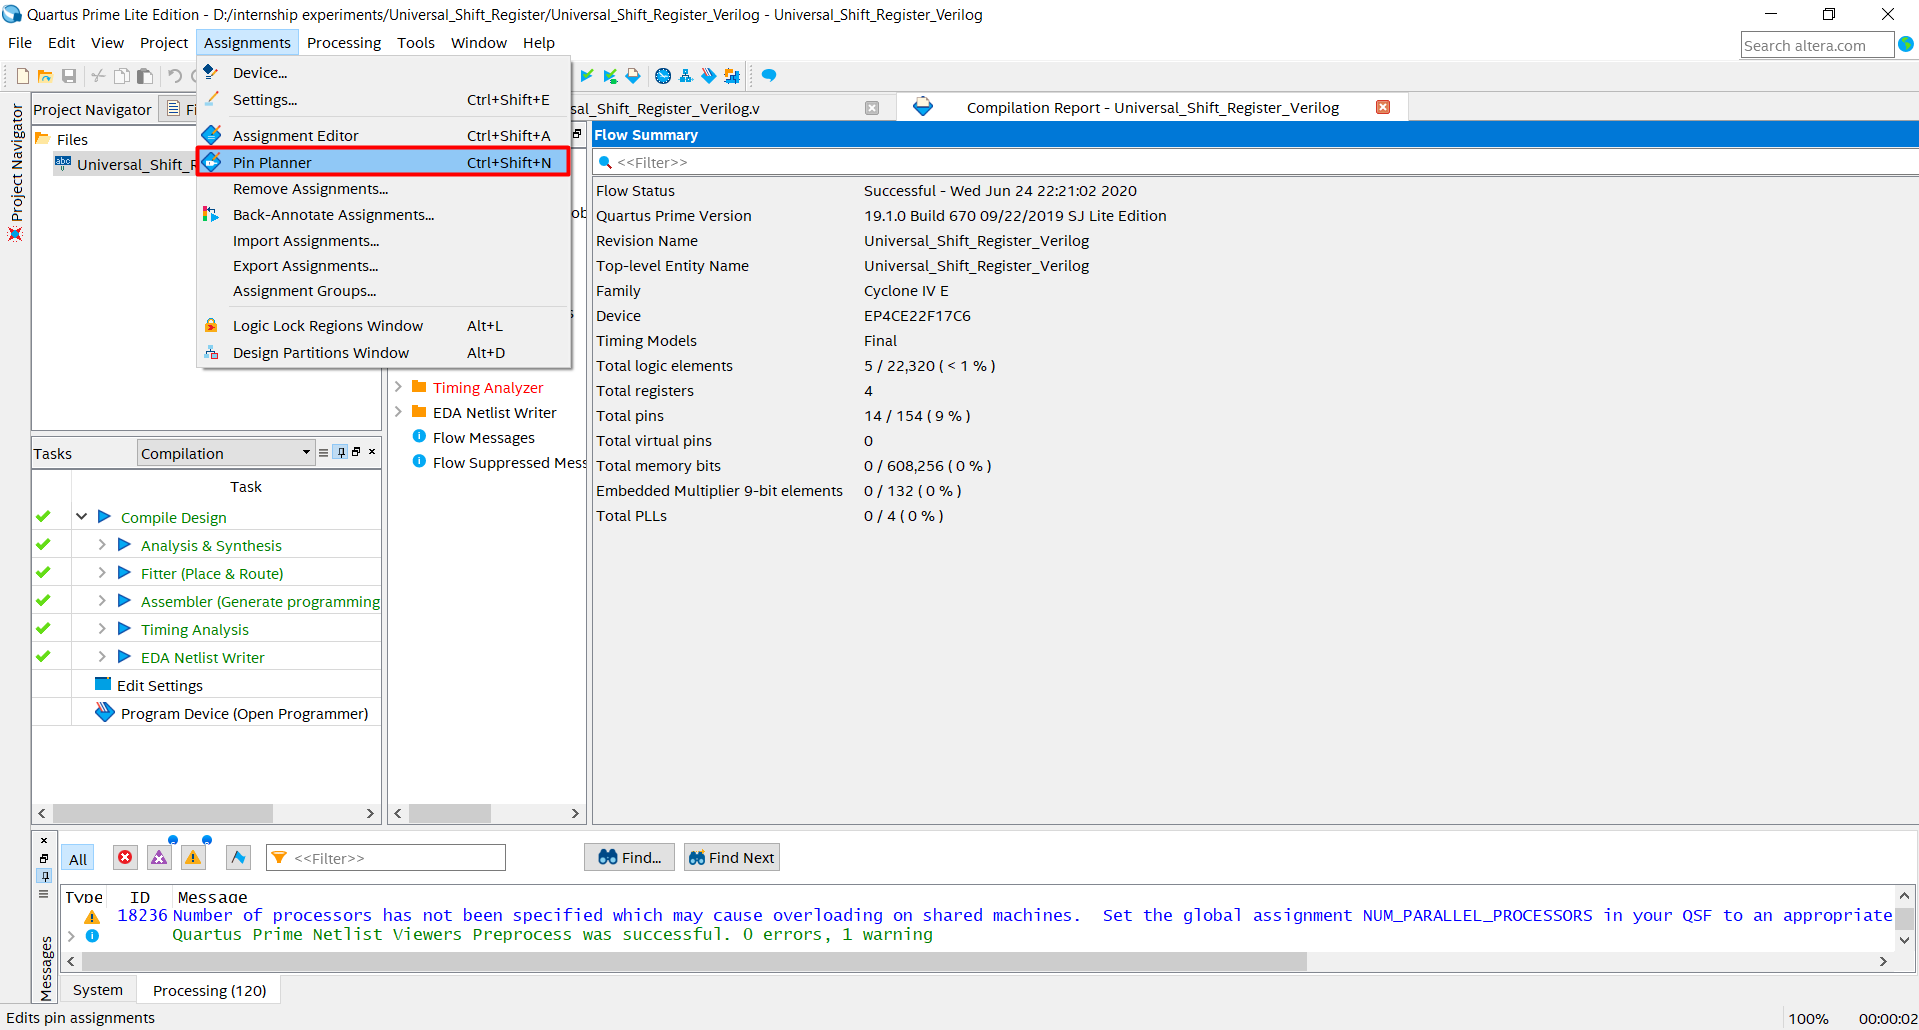
\includegraphics[width=14cm,keepaspectratio]{usr7.png}
        \caption{Opening the PIN PLANNER}
    \end{figure}
    \newpage
    \item Now assign the pins by either dragging and dropping the nodes(\textcolor{blue}{Blue} box) on the required pins(\textbf{Black} box), or click on the drop down menu(\textcolor{red}{Red} box) to search and select a pin. To find out which pin to use, refer the manual of your board. For the DE0-Nano FPGA Board, the manual can be found at \url{https://www.ti.com/lit/ug/tidu737/tidu737.pdf}
     \begin{figure}[H]
        \centering
        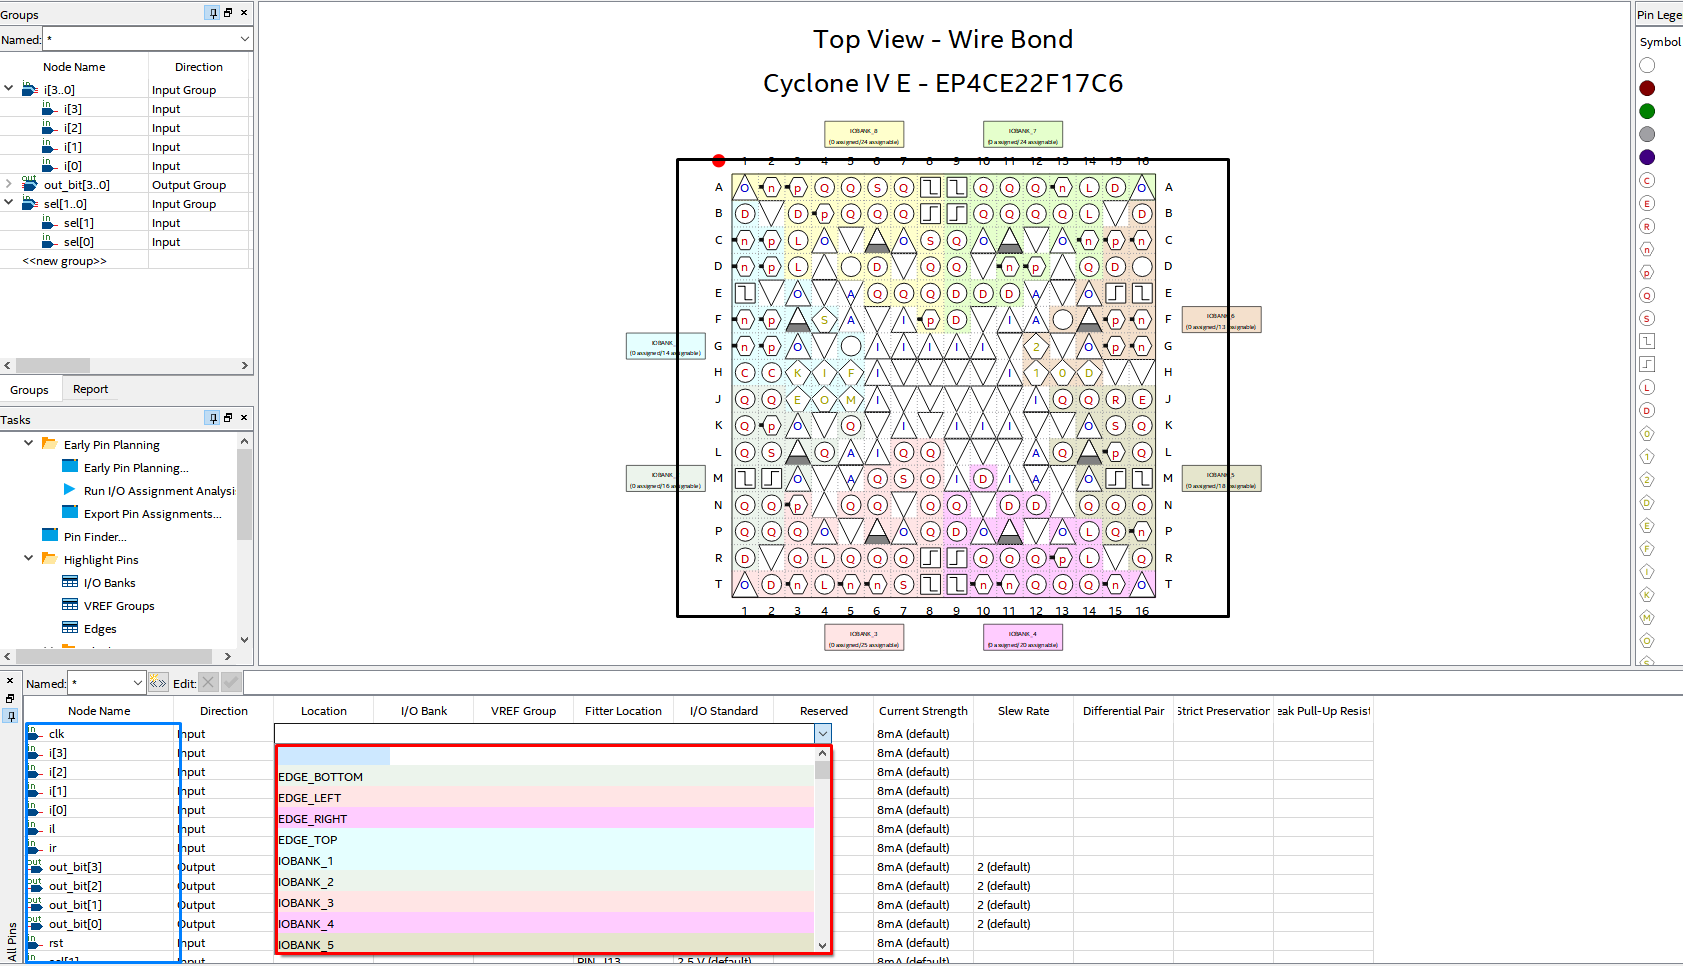
\includegraphics[width=10cm,keepaspectratio]{pin_planner/2.png}
        \caption{Assigning Pins}
    \end{figure}
    
    Here is an example of assigning a pin for the output 'b' in our design
    \begin{figure}[H]
        \centering
        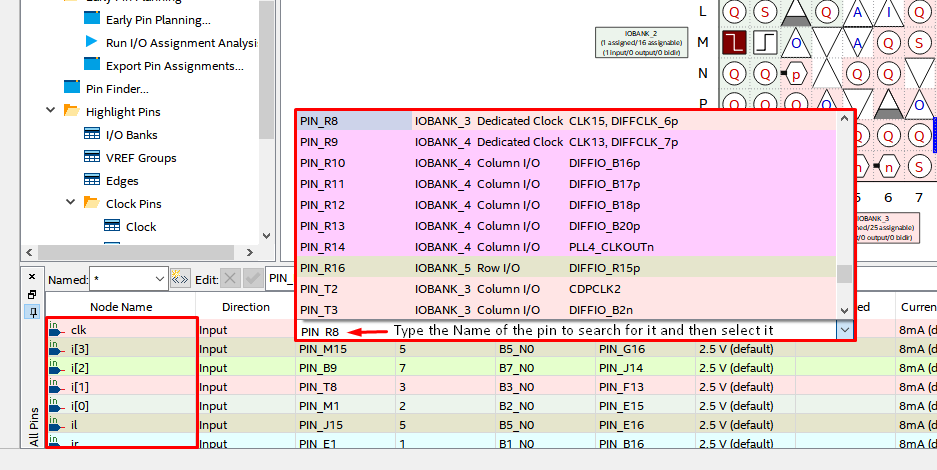
\includegraphics[width=14cm,keepaspectratio]{pin_planner/2_1.png}
        \caption{Assigning pin for b[0]}
    \end{figure}
    \noindent\textbf{Note:}Make sure to select the appropriate I/O standard by referring to the board manual
     \begin{figure}[H]
        \centering
        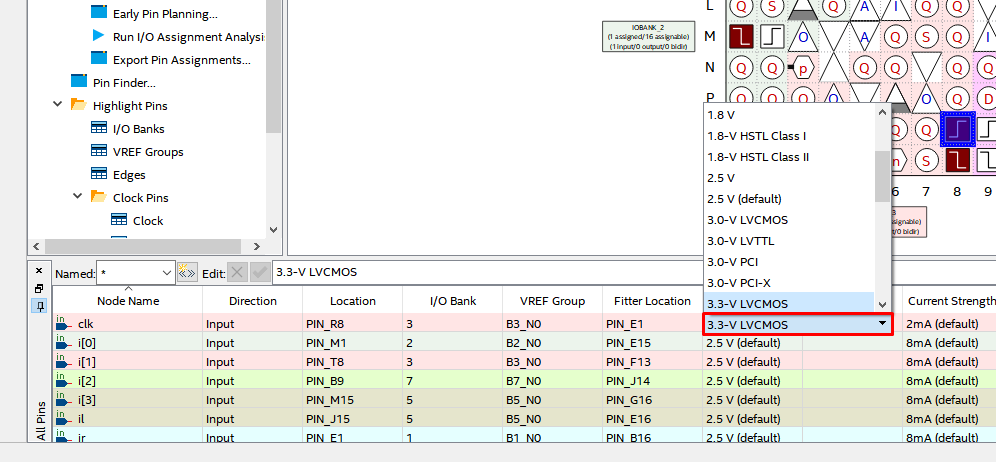
\includegraphics[width=14cm,keepaspectratio]{pin_planner/3.png}
        \caption{Assigning I/O Standards}
    \end{figure}
    
    \item Once all the pins are assigned, Go to \textbf{PROCESSING$\rightarrow$START I/O ASSIGNMENT ANALYSIS}. The analysis checks pin assignments and surrounding logic for illegal assignments and violations of board layout rules.
     \begin{figure}[H]
        \centering
        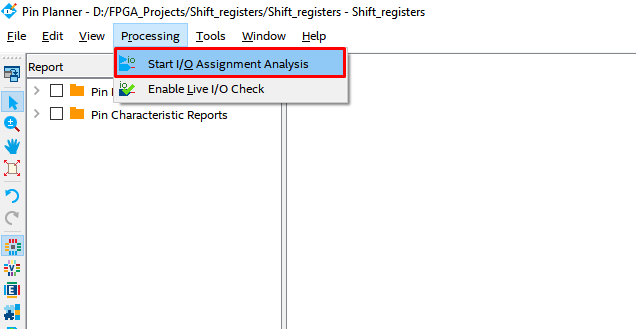
\includegraphics[width=14cm,keepaspectratio]{pin_planner/4.png}
        \caption{Starting the I/O Assignment Analyser}
    \end{figure}
    
\end{enumerate}
\newpage
\section{Downloading the code to DE0 Nano FPGA Board}
 Before starting, Make sure the board is powered on and connected to the computer through an USB Cable. A file with .SOF extension is created during compilation. This file is used to load the program to the board
 
 \begin{enumerate}
     \item Open the programmer by going to 'Tools'$\rightarrow$ 'Programmer'
     \begin{figure}[H]
         \centering
         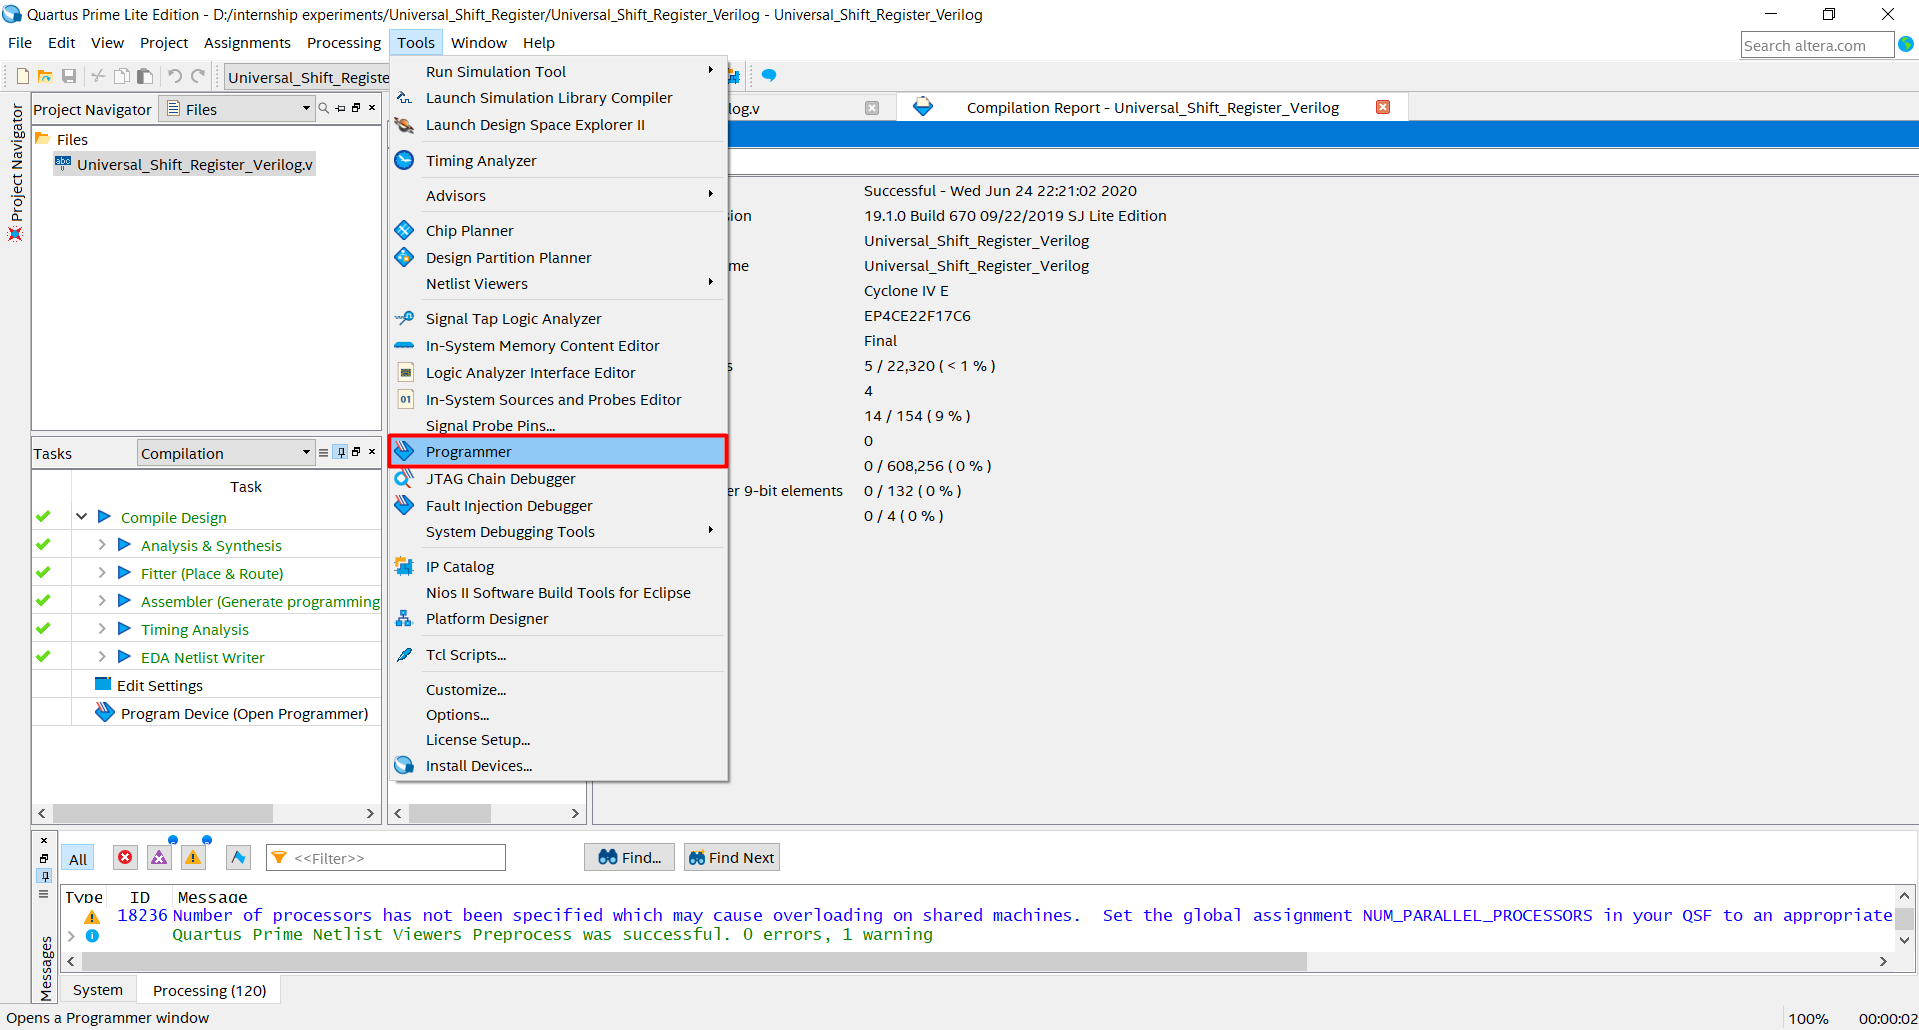
\includegraphics[width=14cm,keepaspectratio]{usr8.png}
         \caption{Opening programmer}
     \end{figure}
     \newpage
     \item Click on hardware setup. The Device required must be listed under "Currently available hardware". If not, check if the device drivers are correctly installed. Choose the hardware from the dropdown menu
     \begin{figure}[H]
         \centering
         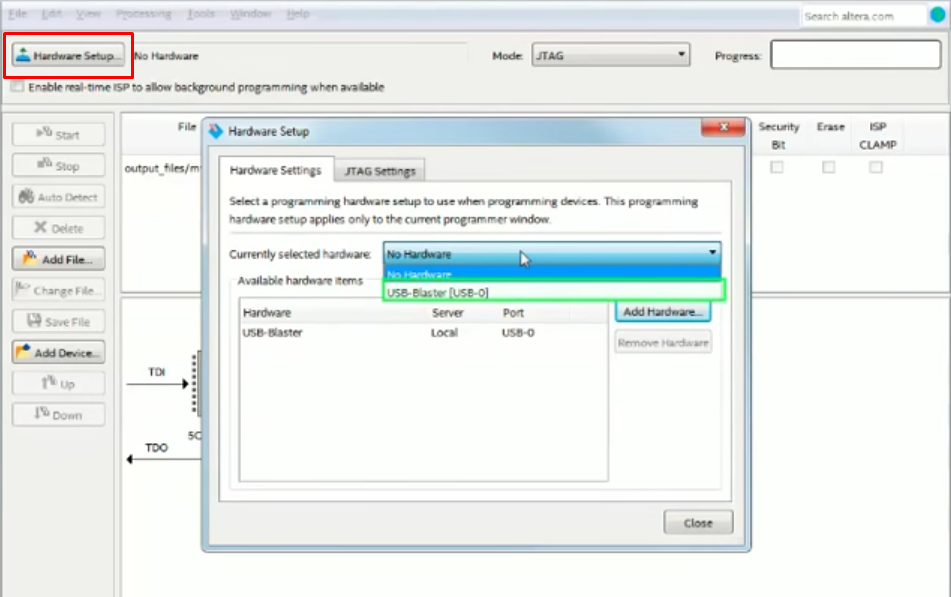
\includegraphics[width=14cm,keepaspectratio]{downloading to board/3.png}
         \caption{Choosing Hardware }

     \end{figure}
     \item If the file is not listed, it can be manually added by clicking on add file. The .SOF file can be found the output directory inside the project directory 
     \begin{figure}[H]
         \centering
         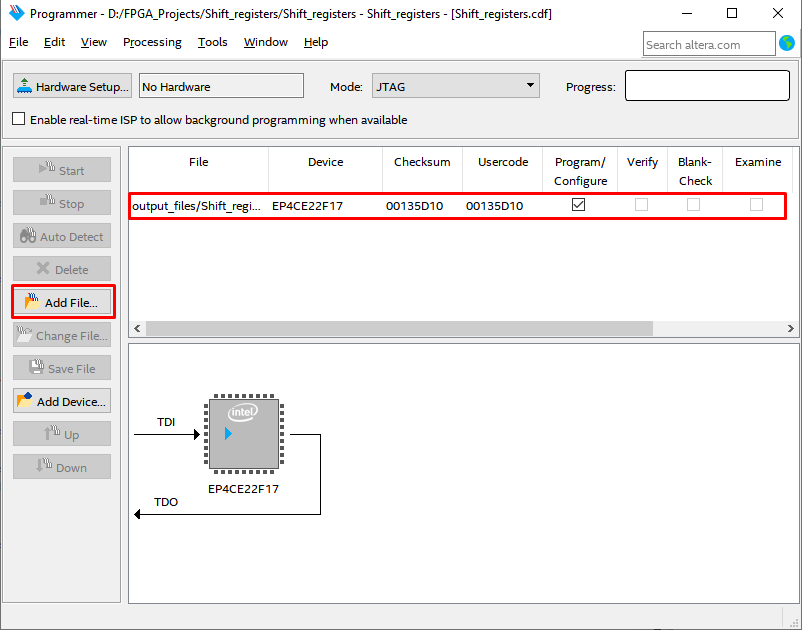
\includegraphics[height=7cm,keepaspectratio]{downloading to board/4.png}
         \caption{Adding file if its not already listed}
     \end{figure}
     \item Make sure the program/configure checkbox is ticked
     \begin{figure}[H]
         \centering
         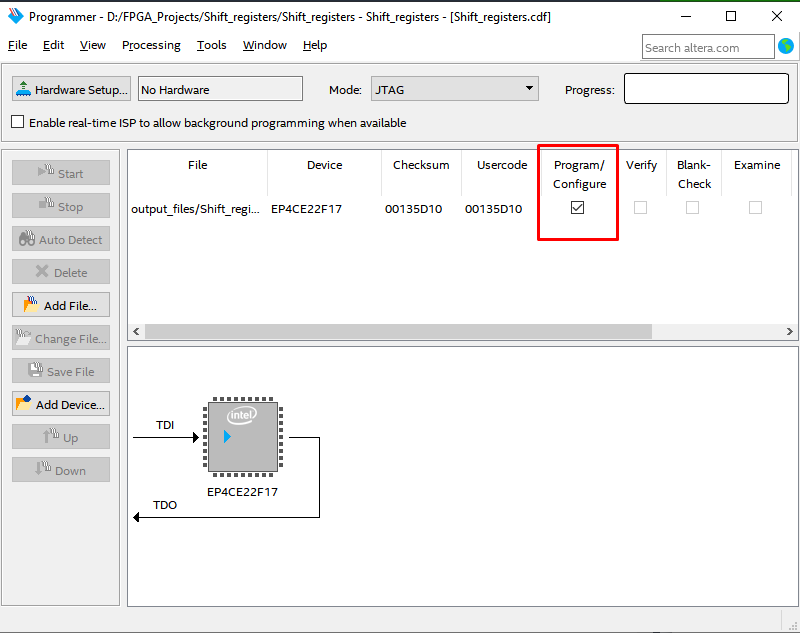
\includegraphics[height=7cm,keepaspectratio]{downloading to board/5.png}
         \caption{Program/Configure is checked}
     \end{figure}
     \item When ready, click on start to start the programming process .'Start' button will be enabled when the 'DEO NANO' board is connected to USB port of your device.
     \textbf{Note:}The start button will be highlighted when the board is connected
     \begin{figure}[H]
         \centering
         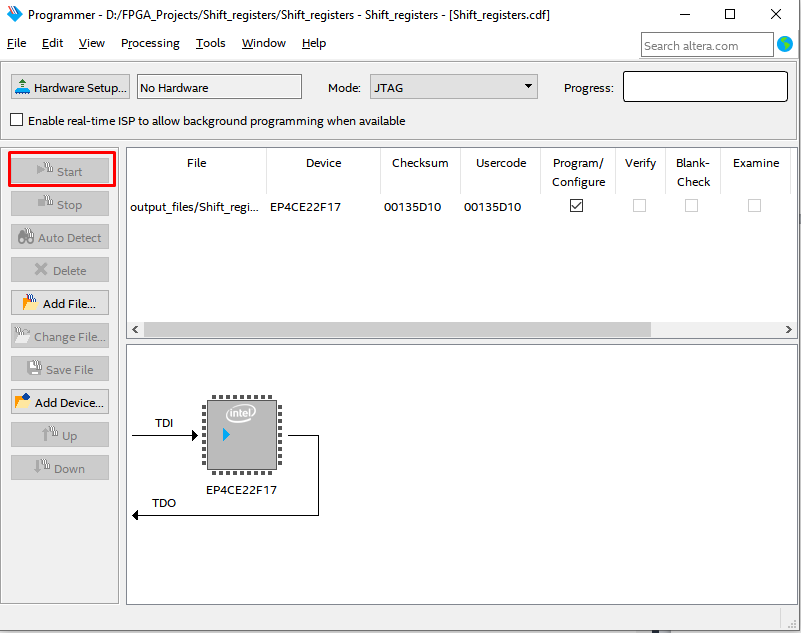
\includegraphics[height=7cm,keepaspectratio]{downloading to board/6.png}
         \caption{Starting the download}
     \end{figure}
     
 \end{enumerate}
 
\section{Implementing in ModelSim}
The TestBench shown here is a Verilog TestBench. For more detailed procedure on using ModelSim, Refer '\textbf{Quick Start Guide to Quartus Prime Lite & ModelSim}' Document
\begin{enumerate}
    \item Create a new verilog file in Quartus Prime
    \begin{figure}[H]
        \centering
        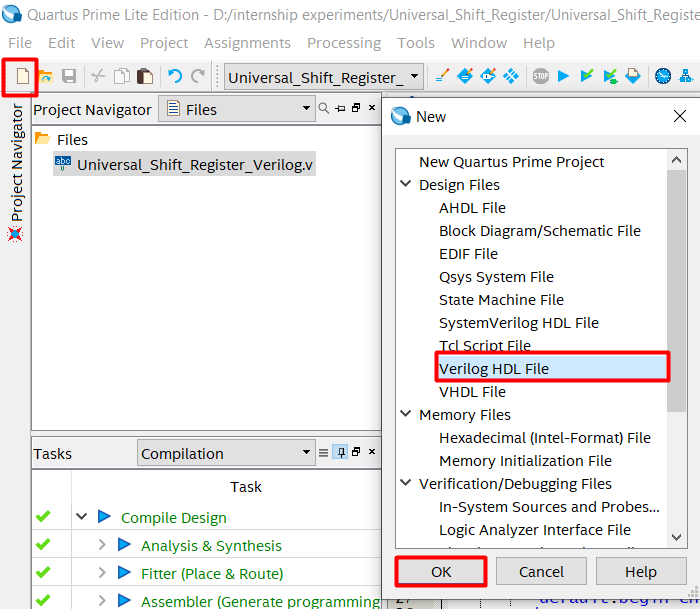
\includegraphics[scale=0.4]{usr9.png}
        \caption{Creating new verilog file}
    \end{figure}
    \item Type in the Testbench code provided in this document and save the file with the same name as the module name
     \begin{figure}[H]
        \centering
        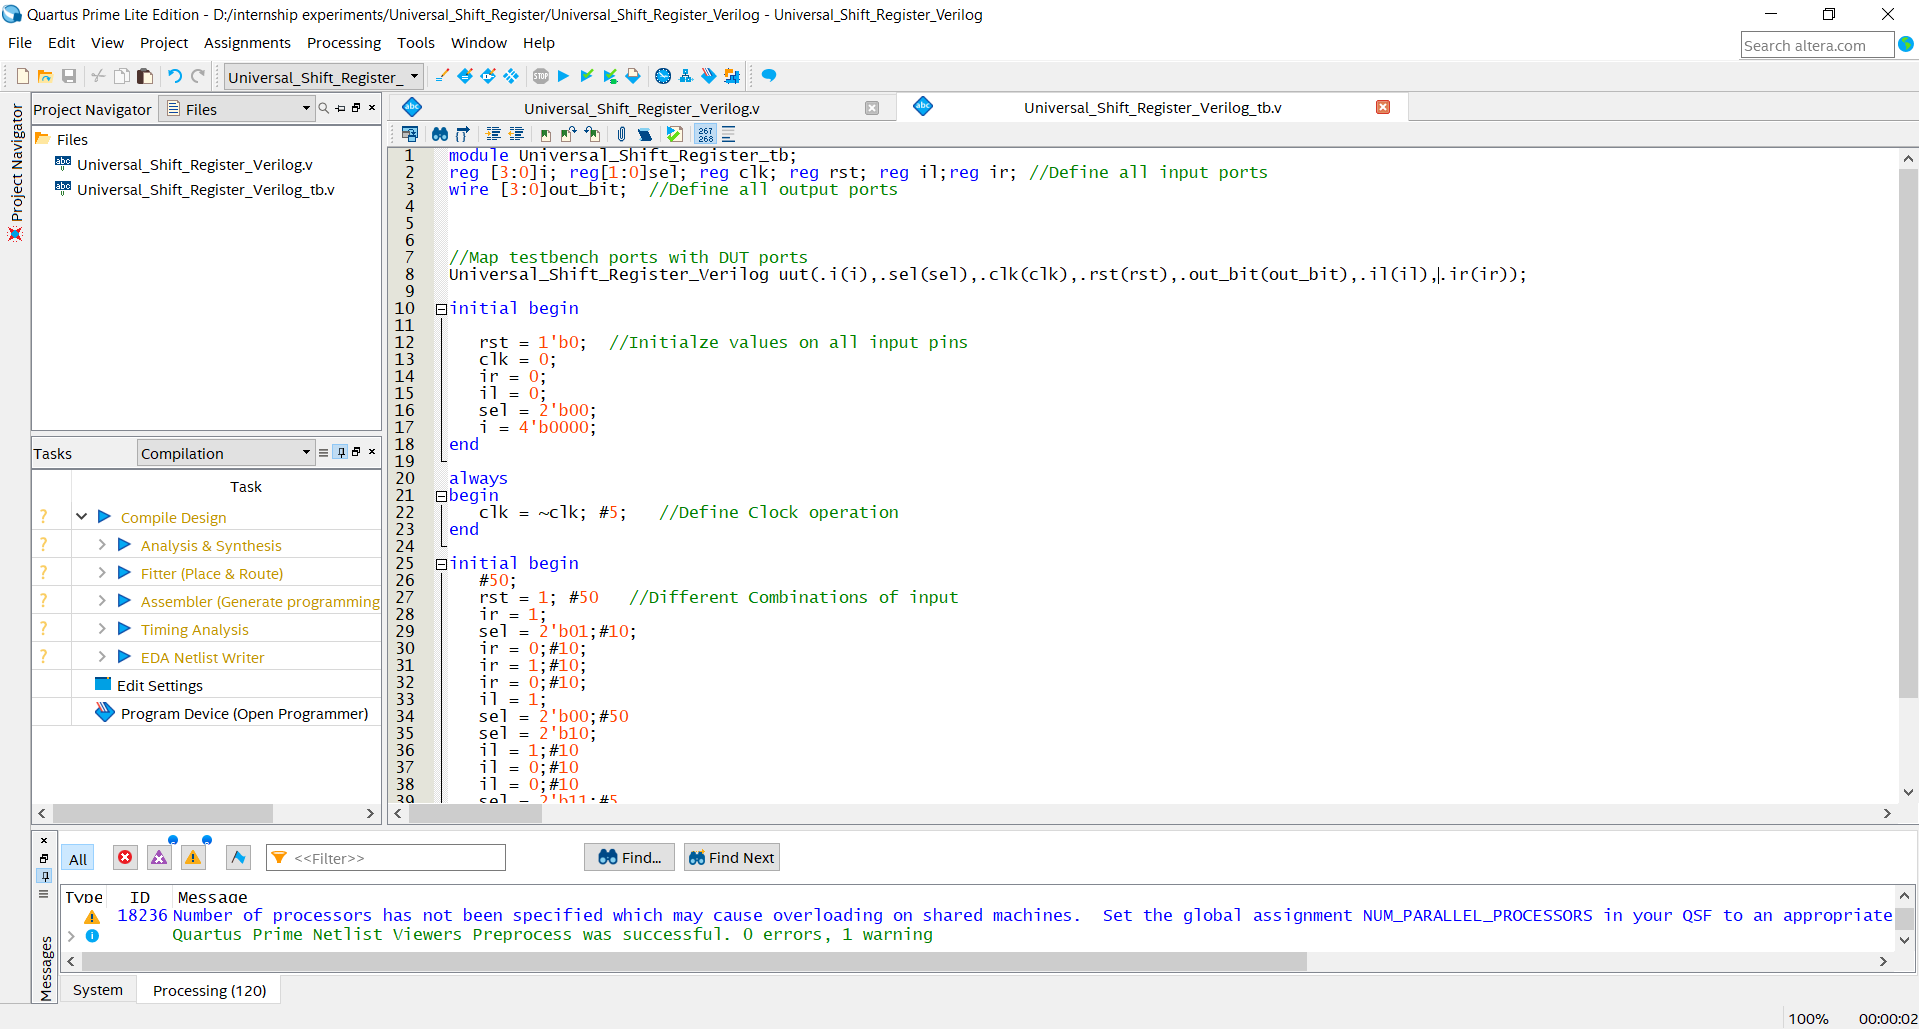
\includegraphics[scale=0.3]{usr10.png}
        \caption{typing the testbench code}
    \end{figure}
    \item Go to \textbf{ASSIGNMENTS$\rightarrow$SETTINGS}
     \begin{figure}[H]
        \centering
         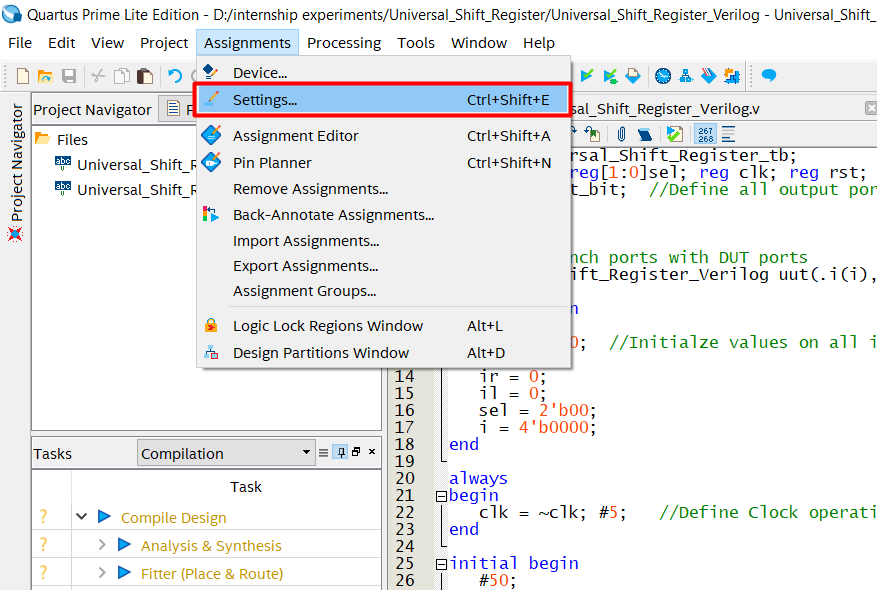
\includegraphics[scale=0.45]{usr11.png}
        \caption{opening settings}
    \end{figure}
    \item Navigate to \textbf{SIMULATION} under \textbf{EDA TOOL SETTINGS}
     \begin{figure}[H]
        \centering
         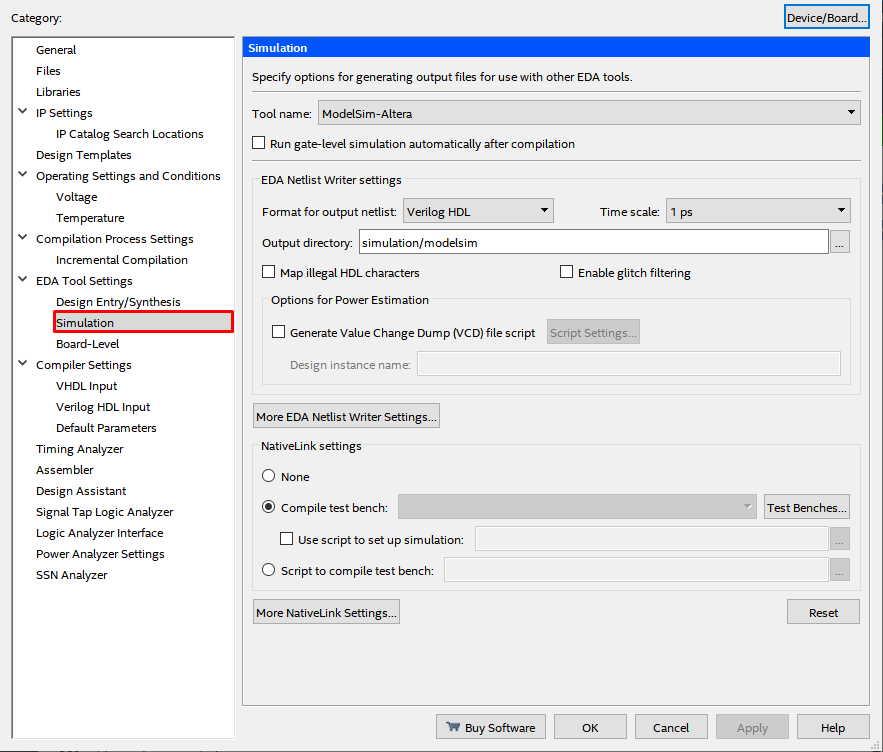
\includegraphics[scale=0.4]{implementing_modelsim/4.png}
        \caption{Navigate to simulation settings}
    \end{figure}
    \item set the language(\textbf{FORMAT FOR OUTPUT NETLIST}) as Verilog HDL. Select \textbf{COMPILE TEST BENCH} and then click on \textbf{TEST BENCHES...}
     \begin{figure}[H]
        \centering
        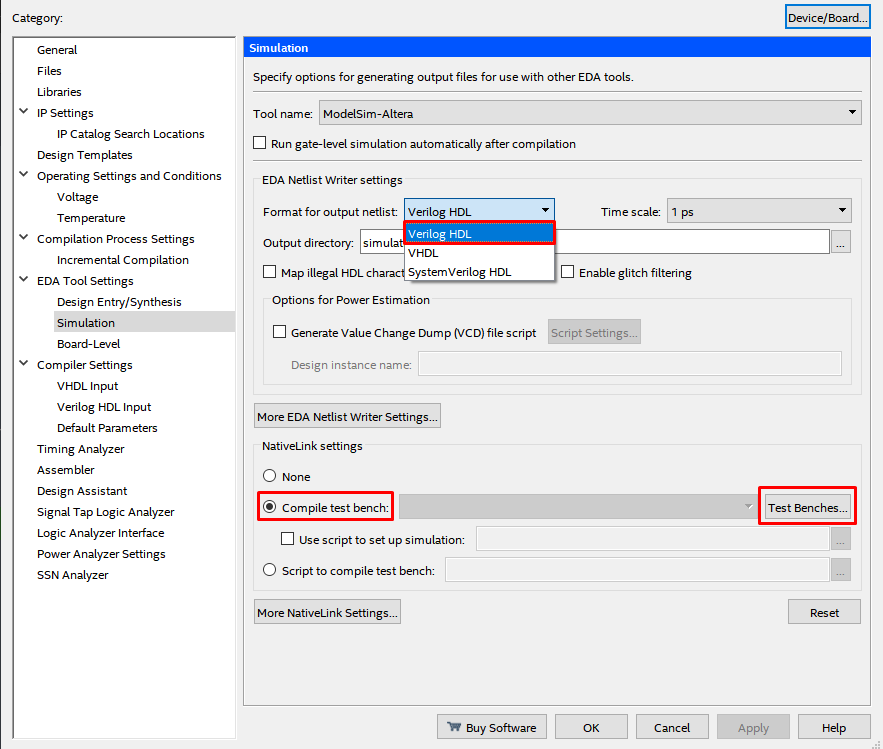
\includegraphics[scale=0.35]{implementing_modelsim/5.png}
        \caption{Configuring the Settings}
    \end{figure}
    \item Click on \textbf{NEW}, this opens another dialogue box. Now type in the testbench name(In this design , its \textbf{Universal\_Shift\_Register\_tb}). Now click on the highlighted browse button
     \begin{figure}[H]
        \centering
         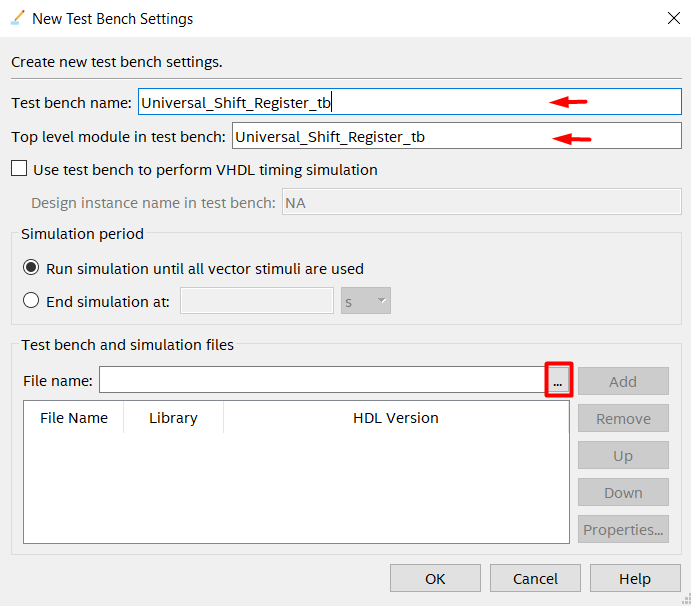
\includegraphics[scale=0.5]{usr12.png}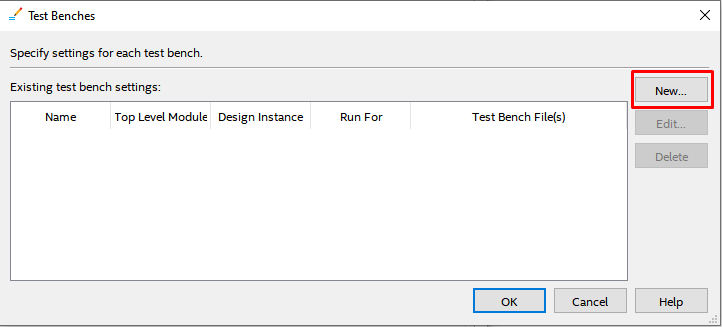
\includegraphics[scale=0.5]{implementing_modelsim/6_1.png}
        \caption{Adding the Tesbench file}
    \end{figure}
    \newpage
    \item Find the testbench file(it can be found in the project directory) and click on \textbf{OPEN}
     \begin{figure}[H]
        \centering
         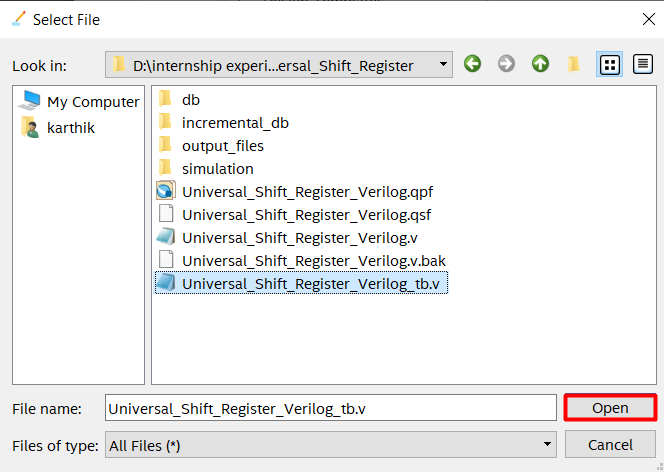
\includegraphics[scale=0.4]{usr13.png}
        \caption{Finding the file in the project directory}
    \end{figure}
    \item Now click on \textbf{ADD},then \textbf{OKAY},then \textbf{OKAY} again and finally click on \textbf{APPLY}
    \textbf{Note:}The \textbf{APPLY} button will be highlighted after \textbf{OKAY} has been clicked on all previous windows
     \begin{figure}[H]
        \centering
         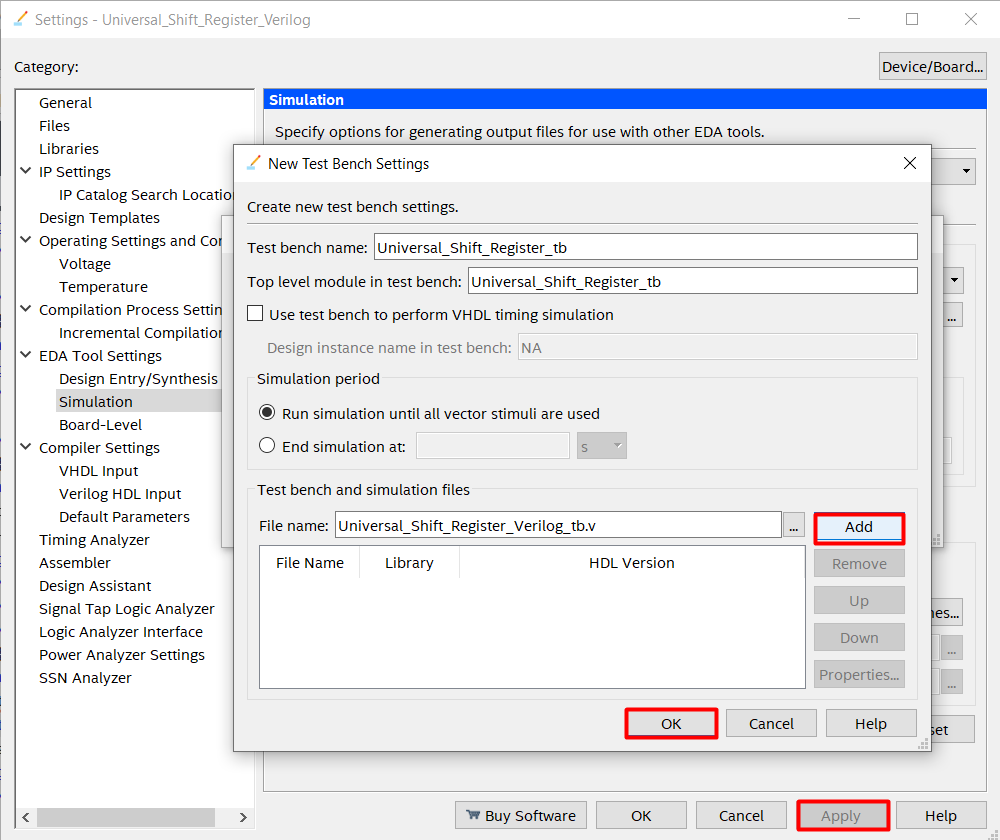
\includegraphics[scale=0.45]{usr14.png}
        \caption{Finalising the testbench adding process}
    \end{figure}
    \newpage
    \item To start the simulation, go to \textbf{TOOLS$\rightarrow$RUN SIMULATION TOOL$\rightarrow$RTL SIMULATION}. This will open ModelSim and display the simulation waveform
     \begin{figure}[H]
        \centering
        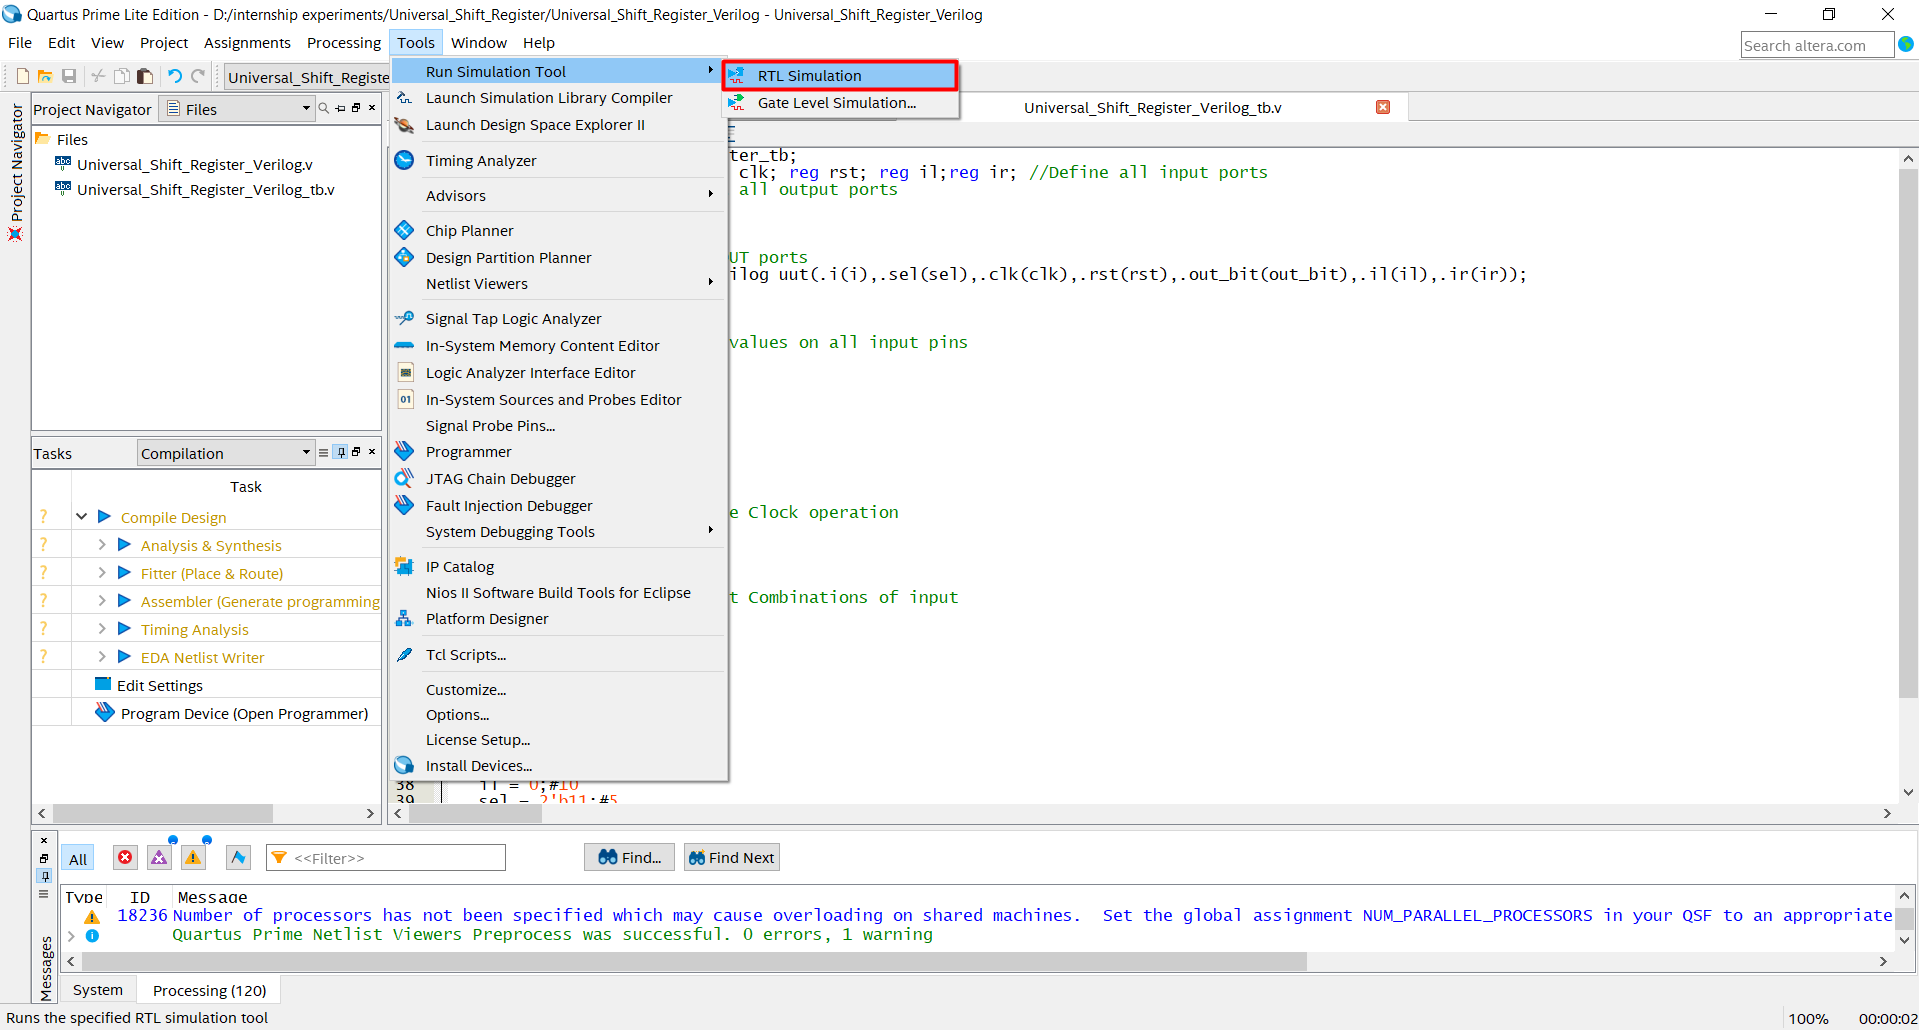
\includegraphics[scale=0.4]{usr15.png}
        \caption{Running the Simulation}
    \end{figure}
\end{enumerate}
\newpage
\section{Simulation Results}
The waveform shown below is the result of the simulation.

\noindent Initially when \textbf{rst=0}, the output is reset to '\textbf{0000}'. After \textbf{50 ns}, \textbf{rst} is set and the register is in normal operation. When \textbf{sel = 00}, the register retains the previous data. At \textbf{0.1 ns}, \textbf{sel=01}, so the shift register is set to \textbf{'Shift right operation'}. At every consecutive clock cycle until \textbf{0.14 ns}, it can be seen that the shift register ouput is shifted right while the MSB is loaded with the value of \textbf{'ir'}. At \textbf{0.14ns}, \textbf{sel=00}, so until \textbf{0.19ns}, the shift register retains the value. At \textbf{0.19 ns}, \textbf{sel=10}, The shift register is set to \textbf{'Shift left Operation'} and at each consecutive clock cycle, the Shift register shifts the data left and loads the LSB with data on the \textbf{'il'} pin. Finally, at \textbf{0.22 ns}, \textbf{sel=11}, this sets the shift register to \textbf{Parellel input mode}, so for every consecutive clock cycle, the shift register is updated with the data on the 4 bit parellel input \textbf{'i'}.
\begin{figure}[H]
    \centering
    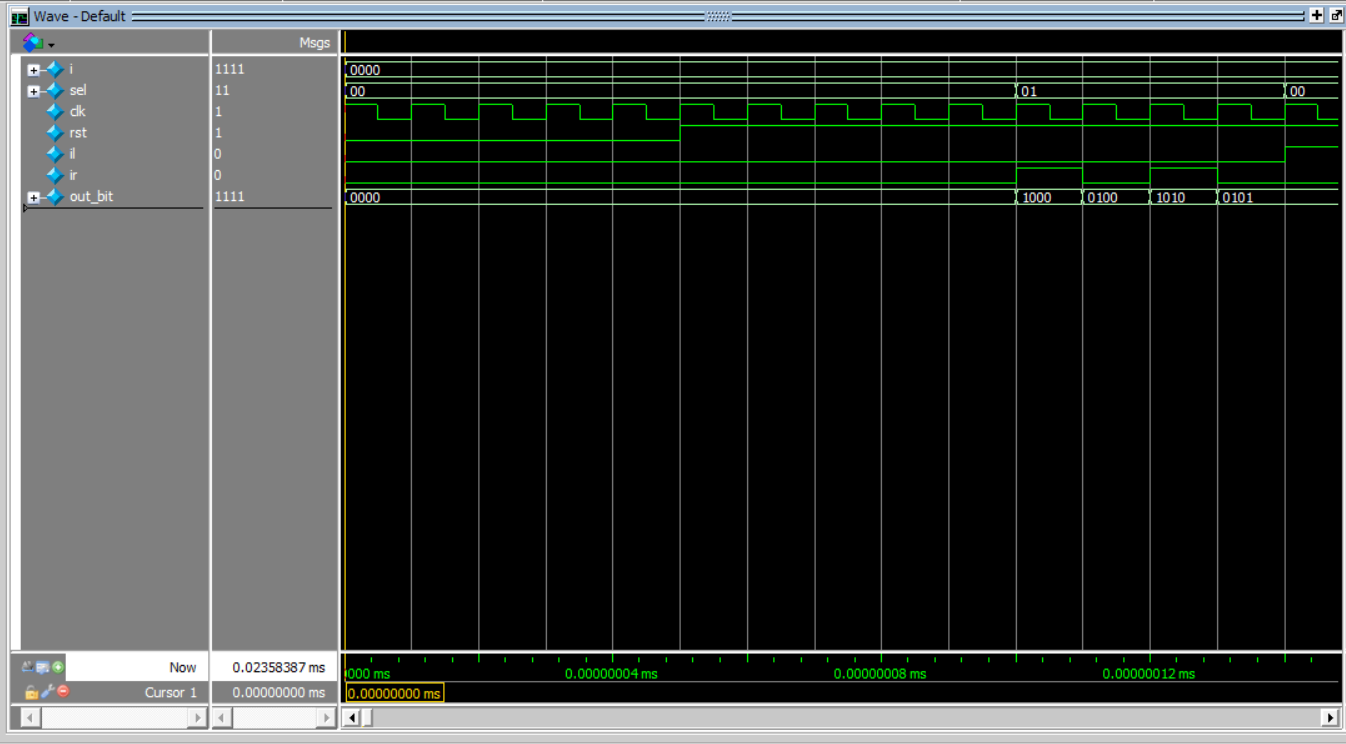
\includegraphics[scale = 0.4]{usrsimu.png}
    \caption{Simulation Waveform}
\end{figure}

%VHDL Code
\newpage
\section{VHDL Code for the Universal Shift Register}
The Entire design can also be implemented using a VHDL code. Irrespective of whether its VHDL or Verilog, the implementation process remains the same
\subsection{RTL Description}
\begin{lstlisting}[style=VHDL, frame=single,linewidth = 17cm]
LIBRARY IEEE;
USE IEEE.STD_LOGIC_1164.ALL;
use IEEE.STD_LOGIC_UNSIGNED.ALL;

ENTITY universal_shift IS
	PORT (
			clock			: IN BIT ;
			clear			: IN BIT ; 
			sl_in			: IN BIT ; 
			sr_in 		: IN BIT ;
			mode 			: IN BIT_VECTOR ( 1 DOWNTO 0 );
			data 			: IN BIT_VECTOR ( 3 DOWNTO 0 );
			q 				: INOUT BIT_VECTOR (3 DOWNTO 0 )
			);
end universal_shift;

ARCHITECTURE behavioural OF universal_shift IS

	BEGIN
	PROCESS (clock, clear)
		BEGIN -- Asynchronous, active-low Clear input:
		IF clear = '0' THEN
		q <= "0000" ; -- Rising edge-triggered D flip-flops:
		
		ELSIF clock'event AND clock = '1' THEN
		
		CASE mode IS
		WHEN "00" => null; 							-- "Do Nothing" mode: retain current flip-flop outputs
		WHEN "01" => q <= (q srl 1) OR (sr_in & "000") ; 	-- Shift Right Serial Input
		WHEN "10" => q <= (q sll 1) OR ("000" & sl_in) ; 	-- Shift Left Serial Input
		WHEN "11" => q <= data ; 									-- Parallel (Broadside) Load
		END case;
	END if;
END process;

END behavioural;
\end{lstlisting}
\newpage
\subsection{TestBench}
\begin{lstlisting}[style=VHDL, frame=single,linewidth = 17cm]
--VHDL Test Bench
--Including Libraries
LIBRARY IEEE;
USE IEEE.STD_LOGIC_1164.ALL;

--Entity Declaration
ENTITY tb_universal_shift IS
END tb_universal_shift;

--Architecture Declaration
ARCHITECTURE behavior OF tb_universal_shift IS
-- Component Declaration for the Unit Under Test (UUT)
COMPONENT universal_shift
	PORT (
			clock			: IN BIT ;
			clear			: IN BIT ; 
			sl_in			: IN BIT ; 
			sr_in 		: IN BIT ;
			mode 			: IN BIT_VECTOR 		( 1 DOWNTO 0 );
			data 			: IN BIT_VECTOR 		( 3 DOWNTO 0 );
			q 				: INOUT BIT_VECTOR 	( 3 DOWNTO 0 )
		);
END COMPONENT;

--Inputs
SIGNAL clear 	: BIT:= '0';
SIGNAL clock 	: BIT:= '0';
SIGNAL sl_in 	: BIT:= '0';
SIGNAL sr_in 	: BIT:= '0';
SIGNAL mode 	: BIT_VECTOR(1 DOWNTO 0) := (OTHERS => '0');
SIGNAL data 	: BIT_VECTOR(3 DOWNTO 0) := (OTHERS => '0');
--Outputs
SIGNAL q			: BIT_VECTOR(3 DOWNTO 0) := (OTHERS => '0');

BEGIN
-- Instantiate the Unit Under Test (UUT)
uut: universal_shift PORT MAP (
					clear=> clear,
					clock => clock,
					sl_in => sl_in,
					sr_in => sr_in,
					mode => mode,
					data => data,
					q => q);
					
\end{lstlisting}\\\newpage
\begin{lstlisting}[style=VHDL, frame=single,linewidth = 17cm]
		-- Clock process definitions
		clk_process :PROCESS
		BEGIN
		clock <= '0';
		WAIT FOR 5 ns;
		clock <= '1';
		WAIT FOR 5 ns;
		END PROCESS;
		-- Stimulus process
		stim_proc: PROCESS
		BEGIN
		--Different Combinations of Input
		clear <= '0';
		WAIT FOR 50 ns;
		clear <= '1';
		sr_in <= '1';
		mode <= "01";
		WAIT FOR 10 ns;
		sr_in <= '0';
		WAIT FOR 10 ns;
		sr_in <= '1';
		WAIT FOR 10 ns;
		sr_in <= '0';
		WAIT FOR 10 ns;
		sl_in <= '1';
		mode <= "00";
		WAIT FOR 50 ns;
		mode <= "10";
		sl_in <= '1';
		WAIT FOR 10 ns;
		sl_in <= '0';
		WAIT FOR 10 ns;
		sl_in <= '0';
		WAIT FOR 10 ns;
		mode <= "11";
		WAIT FOR 5 ns;
		data <= "1111";
		WAIT FOR 100 ns;
		
END PROCESS;
END;
\end{lstlisting}
\end{document}
